\chapter{Results and Discussion}
\label{ch:results}

The results of the experiments conducted in this study are presented in this chapter. The findings are organised according to the experimental design outlined in Section \ref{sec:experimental-setup}. Each section provides a detailed interpretation of the results and their limitations, including relevant figures and tables to support the findings.

\section{General characteristics of storms from the database}

As depicted in Figure \ref{fig:orography_storm_init_end_kde}, the distribution of storm start and end locations are both highly concentrated around the Ethiopian Highlands and diminish quickly closer to the coastline with the Indian Ocean. For the modelling problem, this spatial distribution suggests a strong orographic influence on storm genesis and dissipation.

\begin{figure}[ht]
    \centering
    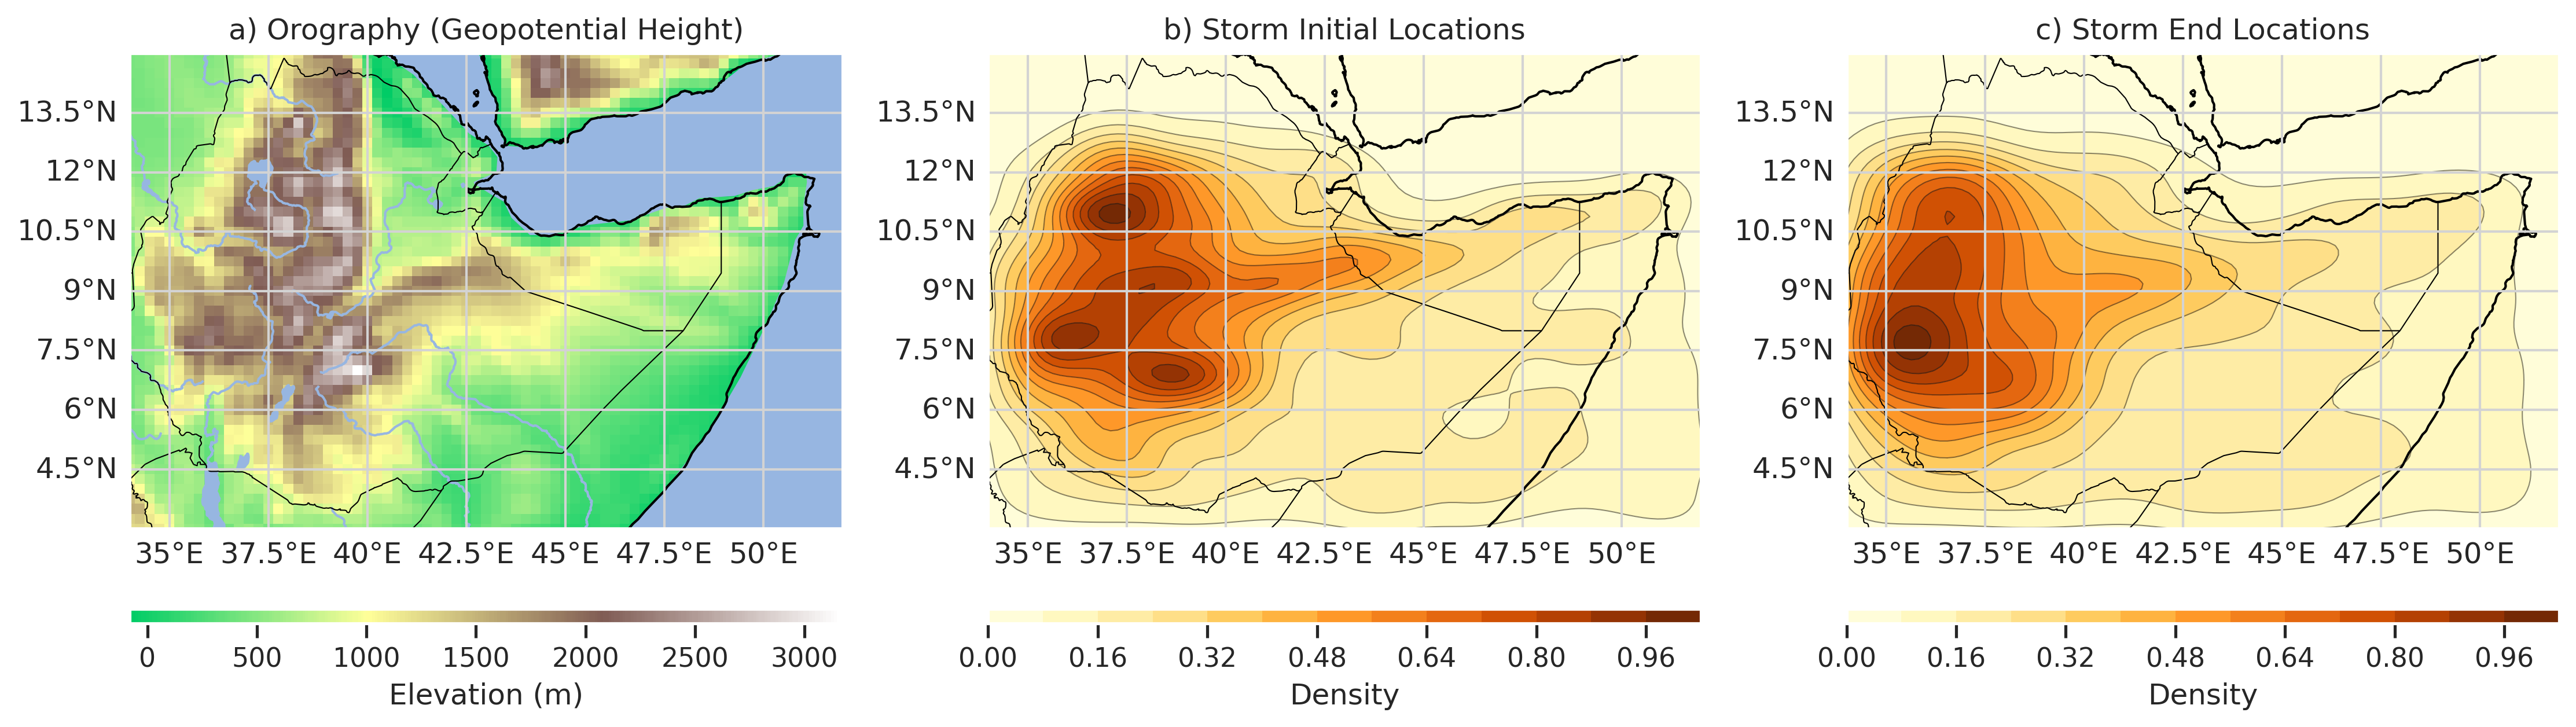
\includegraphics[width=\textwidth]{../figures/generated/exploration/orography_storm_init_end_kde.png}
    \caption{Storm start and end location density plotted geographically alongside elevation. Storms were selected if 1) they lasted longer than 3 hours to precipitation contributions, and 2) their centroids are located within \degN{3} - \degN{15} and \degE{34} - \degE{52} \citep{Hill2023}. See Chapter \ref{ch:method} for details. (a) Elevation over the domain calculated from \acrshort{era5} geopotential height, (b) Storm start location density, (c) Storm end location density.}
    \label{fig:orography_storm_init_end_kde}
\end{figure}

In Figure \ref{fig:orography_storm_init_eat_hours_mode_mean}, the geographic distribution of storm genesis local time is shown. Although the density of storms of the coast of Somalia is limited, it is clear that storms tend to form over the ocean during the early morning hours whereas storms formed over land occur during the late afternoon. This is in agreement with the general understanding of convection over the ocean \citep{Hall1999,Houze2004}. However, orography also appears to play a role pushing genesis later into the night, with clear evening initiations near the strong ridge line at \degE{40} in northeast Ethiopia and around the Abaya Lake valley region. This is potentially due to the influence of mountain-valley breezes which can enhance convection in the late evening and early night hours \citep{Zardi2013}. On average, storms last approximately 5 hours and 15 minutes, and the 95\% percentile of duration is 11 hours.

\begin{figure}[ht]
    \centering
    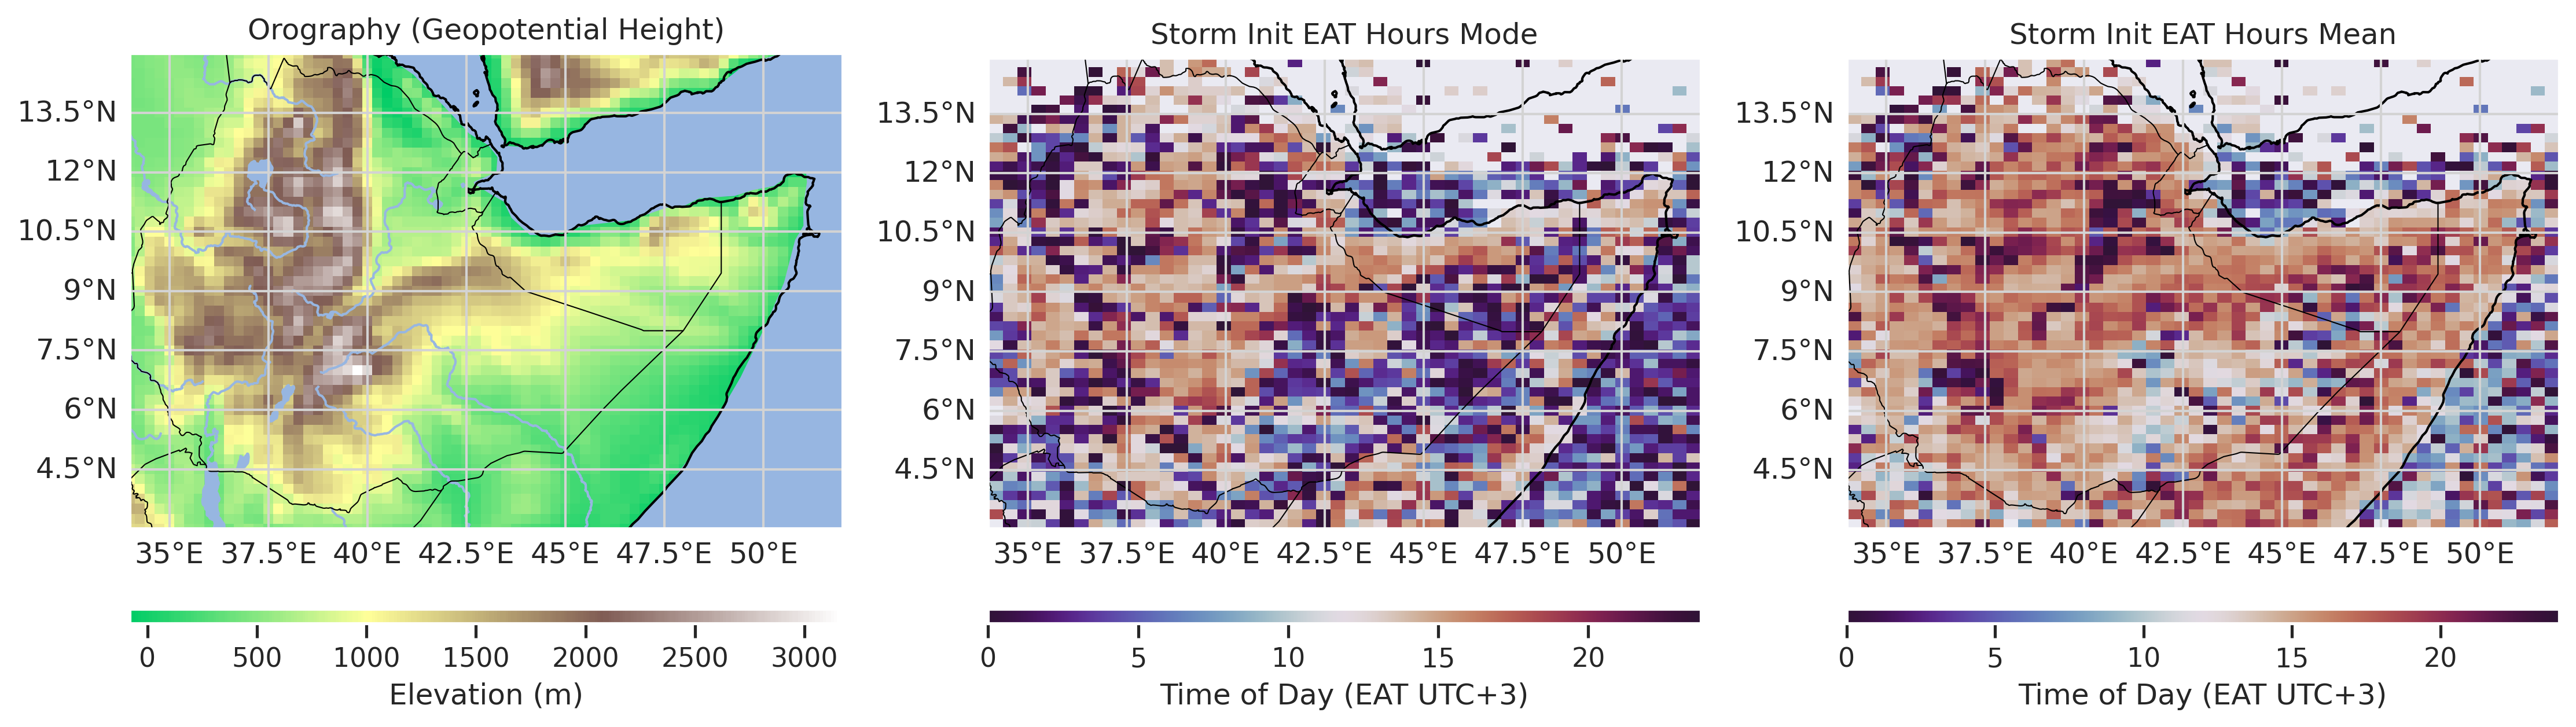
\includegraphics[width=\textwidth]{../figures/generated/exploration/orography_storm_init_eat_hours_mode_mean.png}
    \caption{Storm genesis local time (\acrlong{eat}) plotted geographically alongside elevation. (a) Elevation over the domain calculated from \acrshort{era5} geopotential height, (b) Mean local time of day at which storms initiate, (c) Mode local time of day at which storms initiate.}
    \label{fig:orography_storm_init_eat_hours_mode_mean}
\end{figure}

In Figure \ref{fig:min_bt_over_lifecycle_by_init_type}, the minimum \acrfull{bt} over the lifecycle of storms, categorised by their initiation type is plotted. For this specific analysis, minimum \acrshort{bt} was interpolated over the storm lifecycle and 11 equally spaced points were extracted so as to facilitate comparison across storms of varying durations. Interestingly, on average, storms which initiated over the ocean and during the night tend to be weaker over the entire storm duration. This dynamic may be picked up by the models and should surface in the importance of features like local time (\texttt{eat\_hours}) and the over land flag (\texttt{over\_land}). 

\begin{figure}[ht]
    \centering
    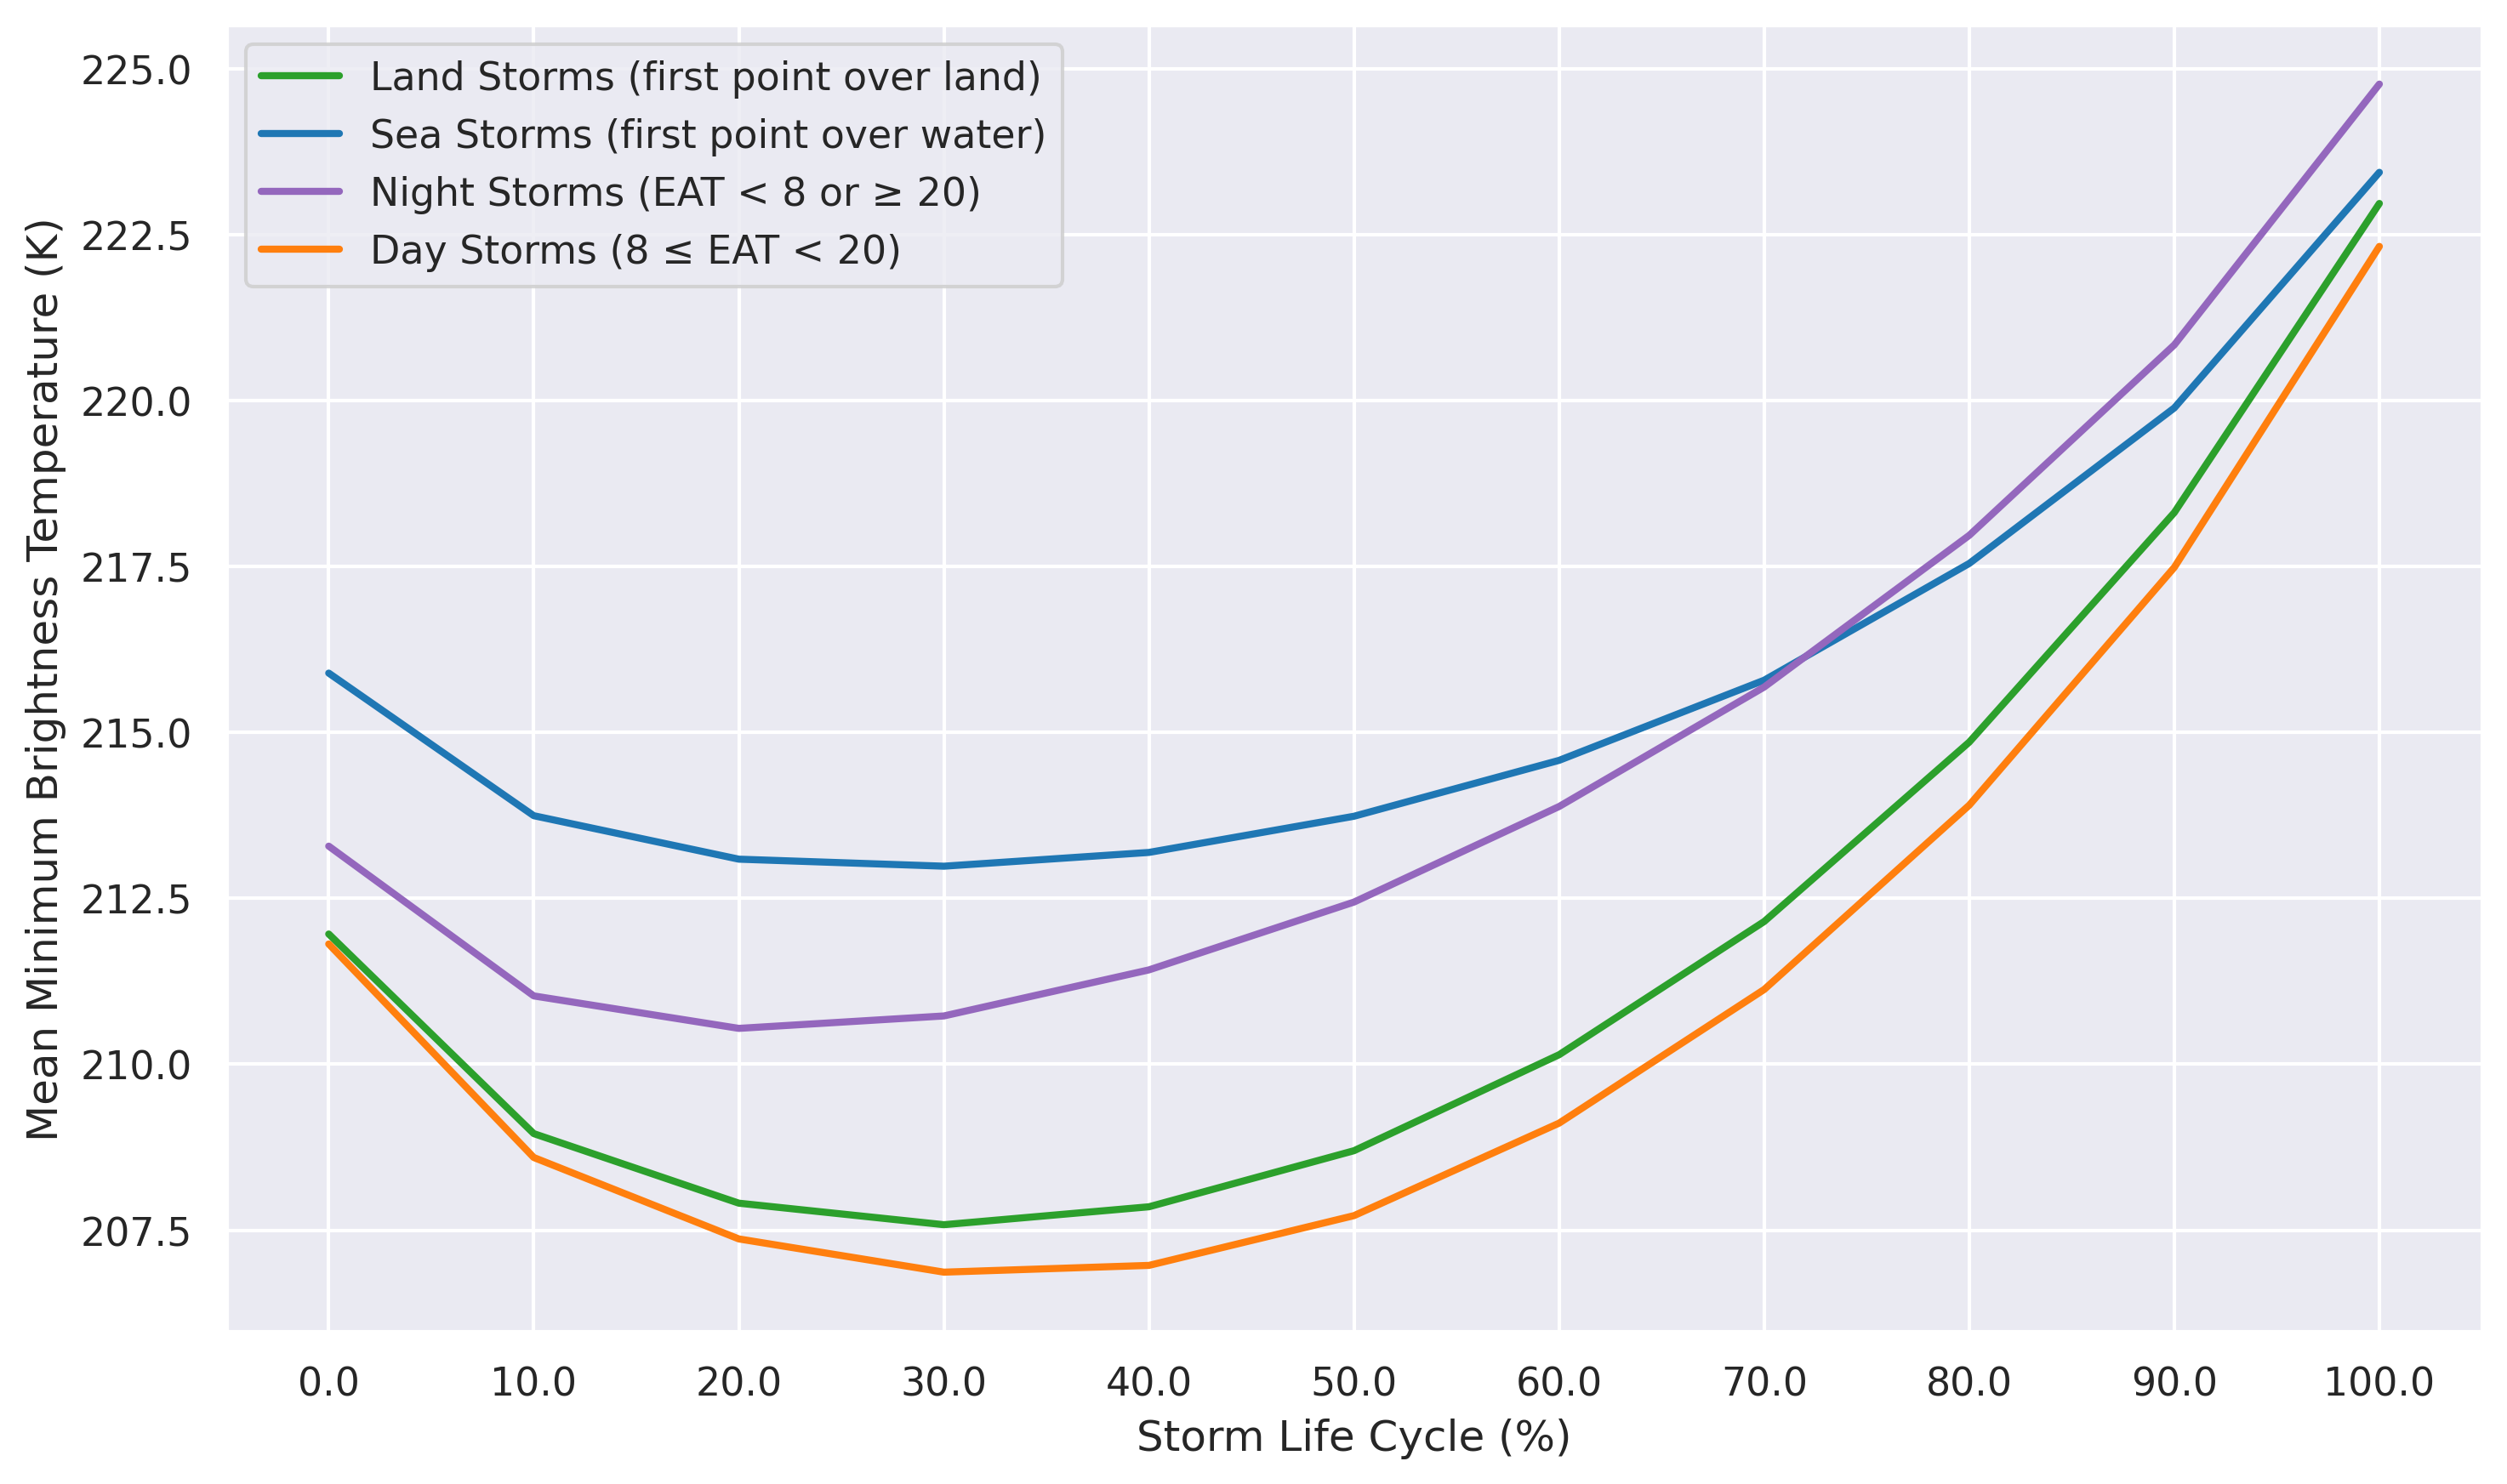
\includegraphics[width=0.7\textwidth]{../figures/generated/exploration/min_bt_over_lifecycle_by_init_type.png}
    \caption{Minimum \acrfull{bt} over the lifecycle of storms, interpolated over storm duration and categorised by storm initiation type.}
    \label{fig:min_bt_over_lifecycle_by_init_type}
\end{figure}

\section{Predict Storm Aggregate Features}

The following two sections provide an overview of the experimental results obtained from the various predictive tasks outlined in Section \ref{sec:experimental-setup}. The experiments in this section aim to predict the overall characteristics of a storm and assess the predictive power of a storm's initial observation.

\subsection{Storm Maximum Intensity}

Table \ref{tab:storm_max_intensity_results} details the performance metrics for storm maximum intensity prediction across the different experimental setups. Note that the target predictand was \texttt{storm\_min\_bt} so lower values indicate a lower overall minimum \acrshort{bt} and thus a stronger \acrshort{mcs}. The standard deviation of the target variable in the respective test sets is also provided as a basis for comparison. If the \acrshort{rmse} of the model is near or above the standard deviation, it has not learned to predict more skilfully than the mean of the target variable.

With comparable \acrshort{rmse} values of $2.7503$ and $2.7610$ over their respective test sets, the result metrics indicate that \acrshort{era5} features alone perform comparably to using all available features. This suggests that the meteorological variables capture most of the relevant information for predicting storm maximum intensity. However, restricting the models to train on only the first observation leads to a substantial drop in performance. For the models trained on all features, the \acrshort{rmse} increases from $4.4872$ to $7.2265$ and for the models trained on \acrshort{era5} features only, the \acrshort{rmse} increases from $4.1072$ to $7.4673$. It should be noted though that the first observations are likely noisy and highly dependent on the storm tracking algorithm and its parameters. Techniques which may compensate for this are further discussed below in Section \ref{sec:results-propagation}. As a result, subsequent explainability analysis will only focus on the all observations models.

\begin{table}[ht]
\centering
\caption{Experimental results for storm maximum intensity prediction.}
\label{tab:storm_max_intensity_results}
\begin{tabular}{|c|c|c|c|c|}
\hline
\multirow{2}{*}{\textbf{Metric}} & \multirow{2}{*}{\textbf{Feature Set}} & \multicolumn{3}{c|}{\textbf{Training Set} } \\ \cline{3-5}
 & & \multicolumn{2}{c|}{\textit{All Observations}} & \textit{First Points Only} \\
\hline \hline
\multirow{2}{*}{\textbf{RMSE} (\unit{\kelvin})} & All & 2.7610 & 4.4872 & 7.2265 \\
 & \acrshort{era5} & 2.7503 & 4.1075 & 7.4673 \\
\hline
\textbf{Target Std} (\unit{\kelvin}) & Both & 9.1679 & 8.8540 & 8.9432 \\
\hline \hline
\multirow{2}{*}{\textbf{Metric}} & \multirow{2}{*}{\textbf{Feature Set}} & \textit{All Points} & \multicolumn{2}{c|}{\textit{First Points}} \\ \cline{3-5}
 & & \multicolumn{3}{c|}{\textbf{Test Set}} \\ 
\hline
\end{tabular}
\end{table}

\begin{figure}[ht]
    \centering
    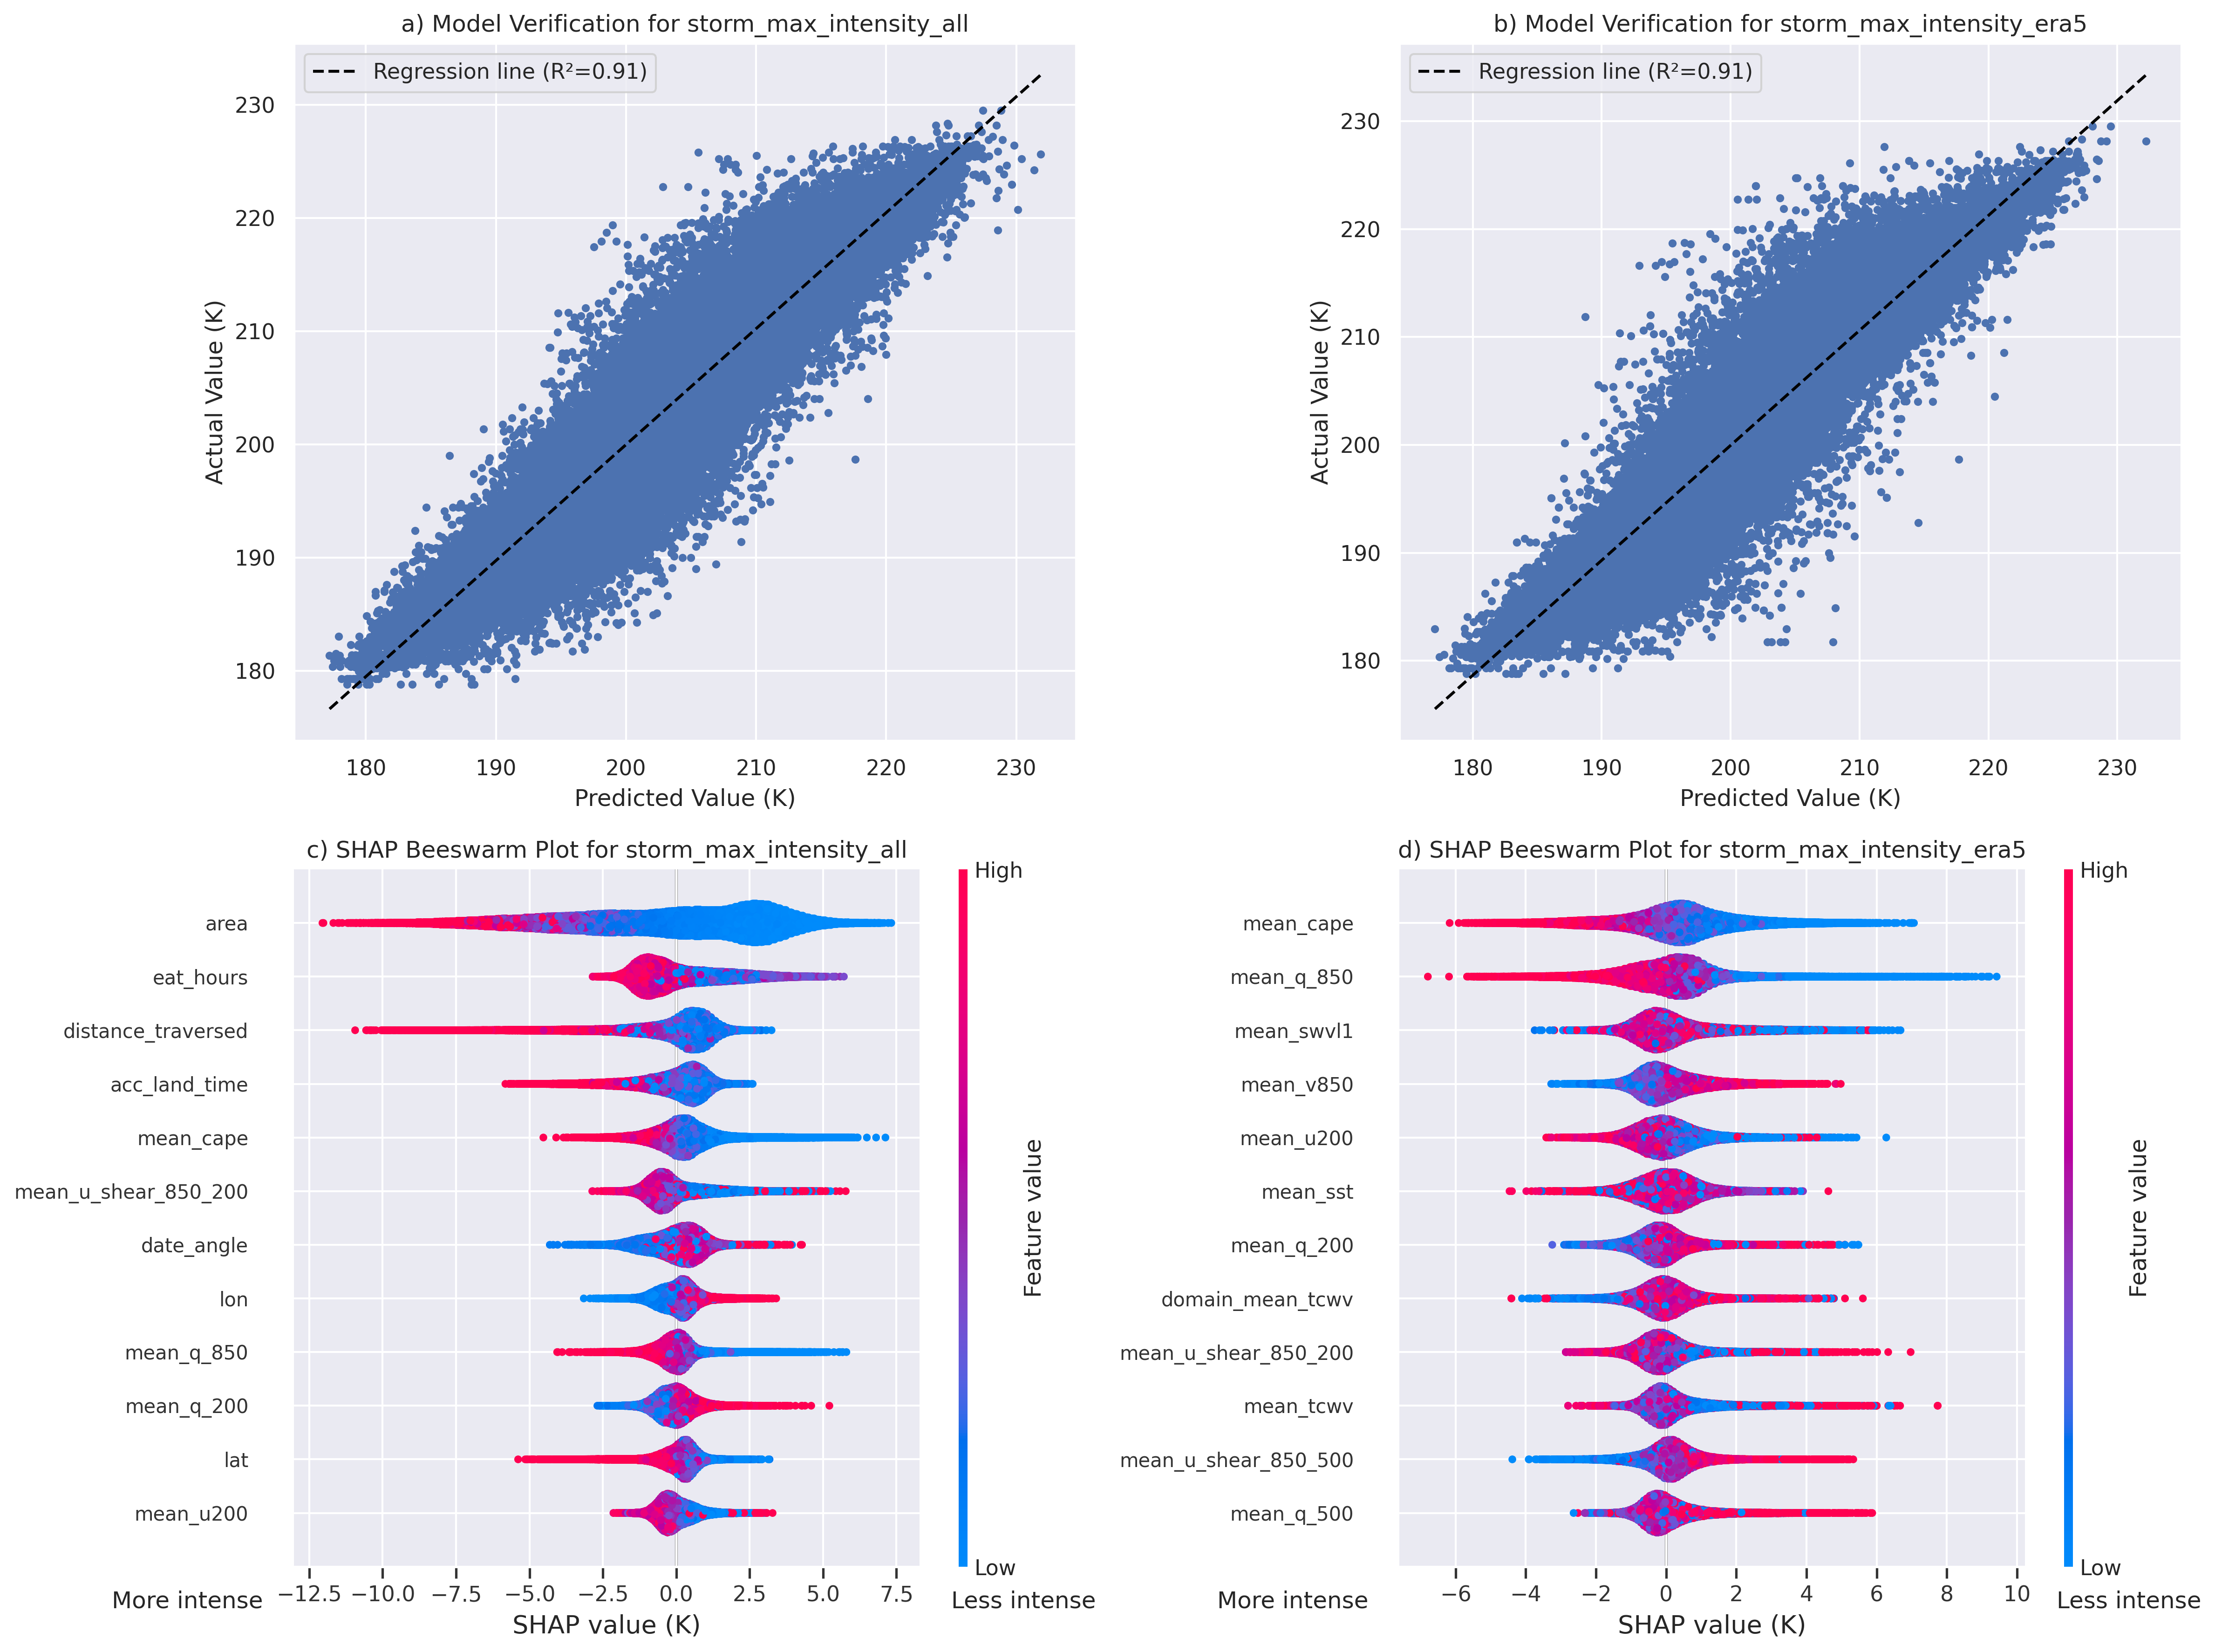
\includegraphics[width=\textwidth]{../figures/generated/experiments/storm_max_intensity/storm_max_intensity_summary.png}
    \caption{Comparison of performance and top features between the models trained on all features and ERA5 data only when predicting storm maximum intensity. Panels (a) and (b) show a comparison between predicted and actual values. The black dashed line shows the line of best fit and the resulting linear correlation coefficient between the actual and predicted values is displayed at the top of the plot. Panels (c) and (d) show top 12 predictors sorted by descending mean \acrshort{shap} value.}
    \label{fig:storm_max_intensity_summary}
\end{figure}

In Figure \ref{fig:storm_max_intensity_summary} a detailed comparison is presented of the model performance and the most influential features for predicting storm maximum intensity using all features versus \acrshort{era5} only. Notably, for the all features model, only one meteorological variable, mean \acrshort{cape}, appears among the top five most important features. The results of the all features model also reveal that stronger storms tend to develop in the late evening (Figure \ref{fig:orography_storm_init_eat_hours_mode_mean}, panel (c) \texttt{eat\_hours}). Across both models, \acrshort{cape} consistently emerges as the most important meteorological factor.

Particularly striking for these models is that the importance of low-level meridional winds changes with time of day, date, and location. Figure \ref{fig:storm_max_intensity_era5_shap_mean_v850_map_by_month} illustrates this variability over the study region throughout the year. During the summer months, strong southerlies are observed on the Somali coastal plains, which correspond to positive \acrshort{shap} values, meaning that these southerlies hinder \acrshort{mcs} intensity. In the winter months, the influence tends to be negative or neutral over the entire domain.

\begin{figure}[ht]
    \centering
    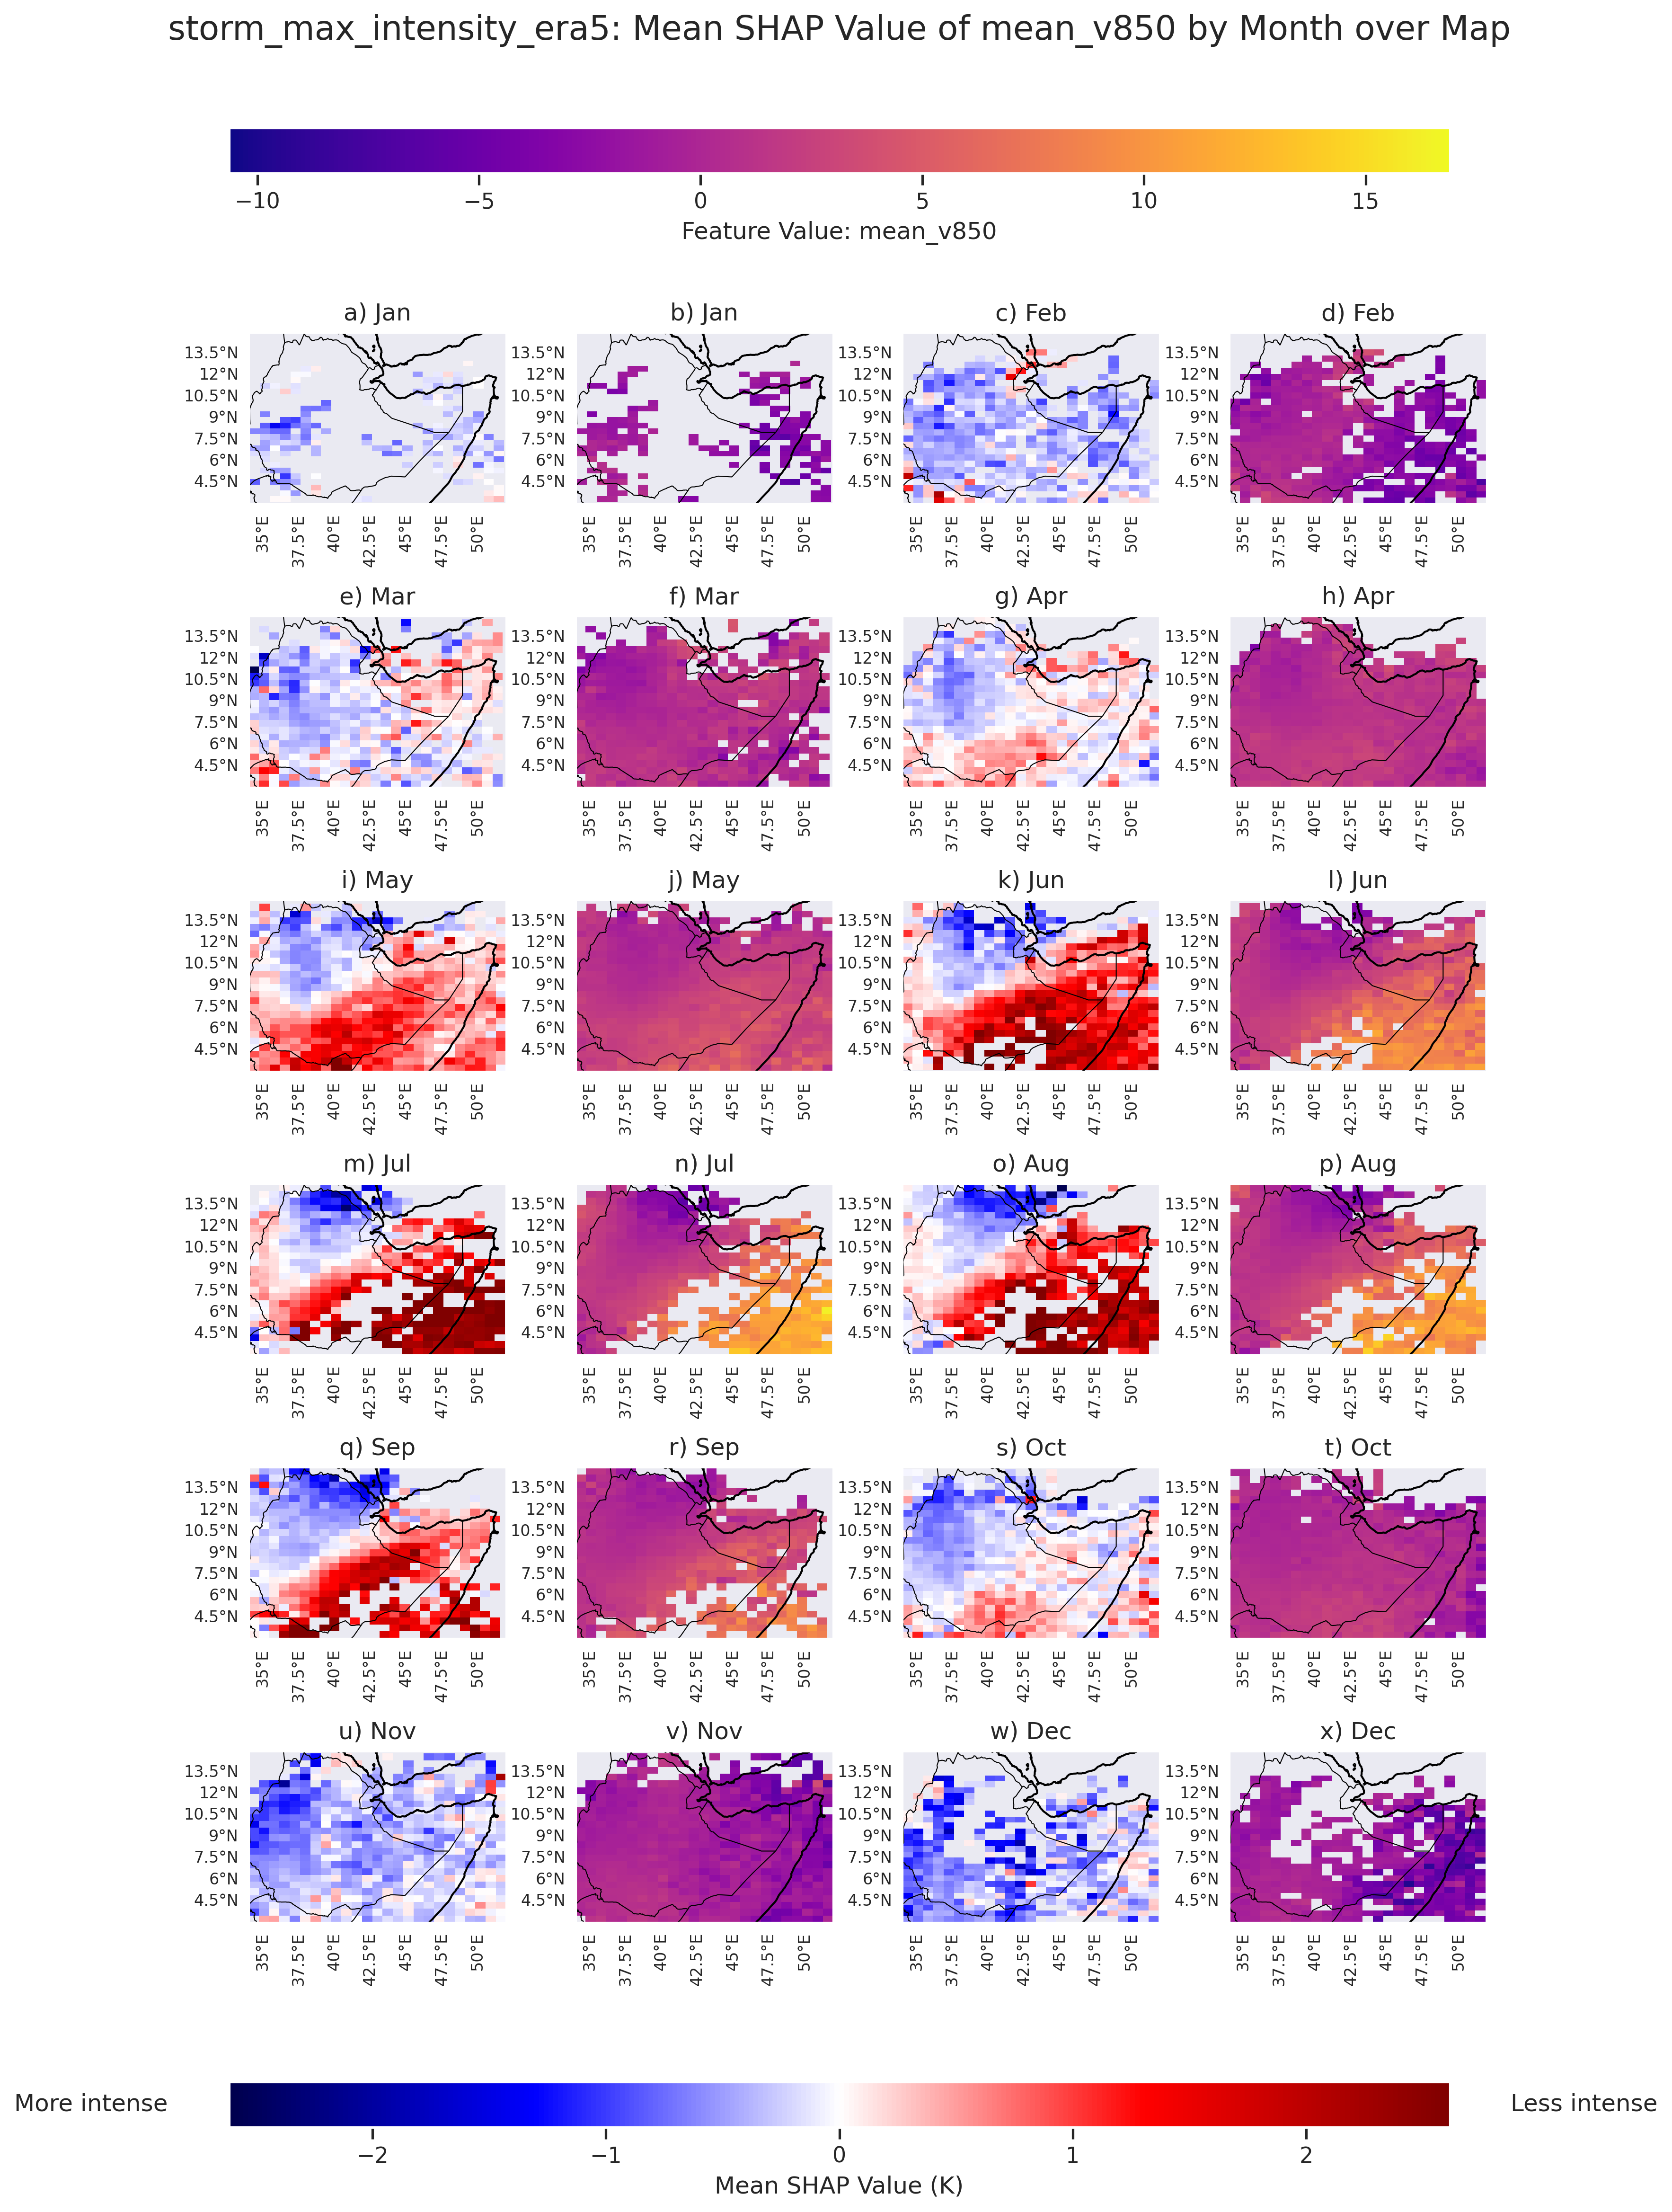
\includegraphics[width=\textwidth]{../figures/generated/experiments/storm_max_intensity/geographic_corr/storm_max_intensity_era5_shap_mean_v850_map_by_month.png}
    \caption{Feature contribution of \SI{850}{\hecto\pascal} meridional wind over East Africa by month for storm maximum intensity prediction using \acrshort{era5} features. Plots are paired by month to compare mean \acrshort{shap} values (left) with feature values (right). For example, panel (a) shows mean \acrshort{shap} values for \SI{850}{\hecto\pascal} meridional wind for January measured in the units of the target variable (\unit{\kelvin}) and panel (b) shows the respective feature values for \SI{850}{\hecto\pascal} meridional wind for January in \unit{\meter\per\second}.}
    \label{fig:storm_max_intensity_era5_shap_mean_v850_map_by_month}
\end{figure}

\clearpage
\subsection{Storm Direction}

Table \ref{tab:storm_direction_results} details the performance metrics for storm direction prediction across different experimental setups. Surprisingly, the models trained on the \acrshort{era5} features set slightly outperform those trained on all features. For models trained on all observations, the \acrshort{rmse} is $19.0178$ and $21.7822$ respectively when comparing the two feature sets. For models trained only on the first points, the \acrshort{rmse} increases to $49.8792$ and $49.5919$. Finally, evaluating the model trained on all observations against the test set of only first points, the \acrshort{rmse} increases to $32.7166$ and $30.3470$. The models trained on all observations are reasonably skilful with the \acrshort{era5} features set performing slightly better, but those trained only on first points are not. As such, subsequent explainability analysis will focus only on the all observations models due to the poor performance of the first points only models.

\begin{table}[ht]
\centering
\caption{Experimental results for storm direction prediction}
\label{tab:storm_direction_results}
\begin{tabular}{|c|c|c|c|c|}
\hline
\multirow{2}{*}{\textbf{Metric}} & \multirow{2}{*}{\textbf{Feature Set}} & \multicolumn{3}{c|}{\textbf{Training Set} } \\ \cline{3-5}
 & & \multicolumn{2}{c|}{\textit{All Observations}} & \textit{First Points Only} \\
\hline \hline
\multirow{2}{*}{\textbf{RMSE} (\unit{\degree})} & All & 21.7822 & 32.7166 & 49.8792 \\
 & \acrshort{era5} & 19.0178 & 30.3470 & 49.5919 \\
\hline
\textbf{Target Std} (\unit{\degree}) & Both & 61.3066 & 61.6789 & 64.1756 \\
\hline \hline
\multirow{2}{*}{\textbf{Metric}} & \multirow{2}{*}{\textbf{Feature Set}} & \textit{All Points} & \multicolumn{2}{c|}{\textit{First Points}} \\ \cline{3-5}
 & & \multicolumn{3}{c|}{\textbf{Test Set}} \\ 
\hline
\end{tabular}
\end{table}

For better context in interpreting the meaning of the \acrshort{shap} values, the distribution of storm cardinal directions in the dataset is shown as a radar plot in Figure \ref{fig:storm_cardinal_directions_distribution}. The distribution indicates that the majority of storms move in a westerly direction and indeed the mean storm direction is approximately \ang{258}. Thus, generally for this experiment, positive \acrshort{shap} values can be interpreted as shifting the predicted storm direction northward, while negative values indicate a southward shift.

\begin{figure}[ht]
    \centering
    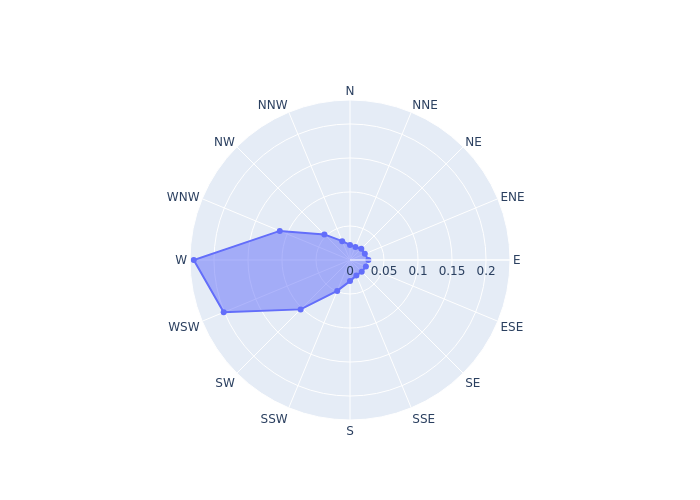
\includegraphics[width=0.6\textwidth]{../figures/generated/exploration/storm_cardinal_directions_distribution.png}
    \caption{Distribution of storm cardinal directions in the dataset. The radius of each point is equal to the proportion of storms in the database whose overall direction is closest to that cardinal direction.}
    \label{fig:storm_cardinal_directions_distribution}
\end{figure}

\begin{figure}[ht]
    \centering
    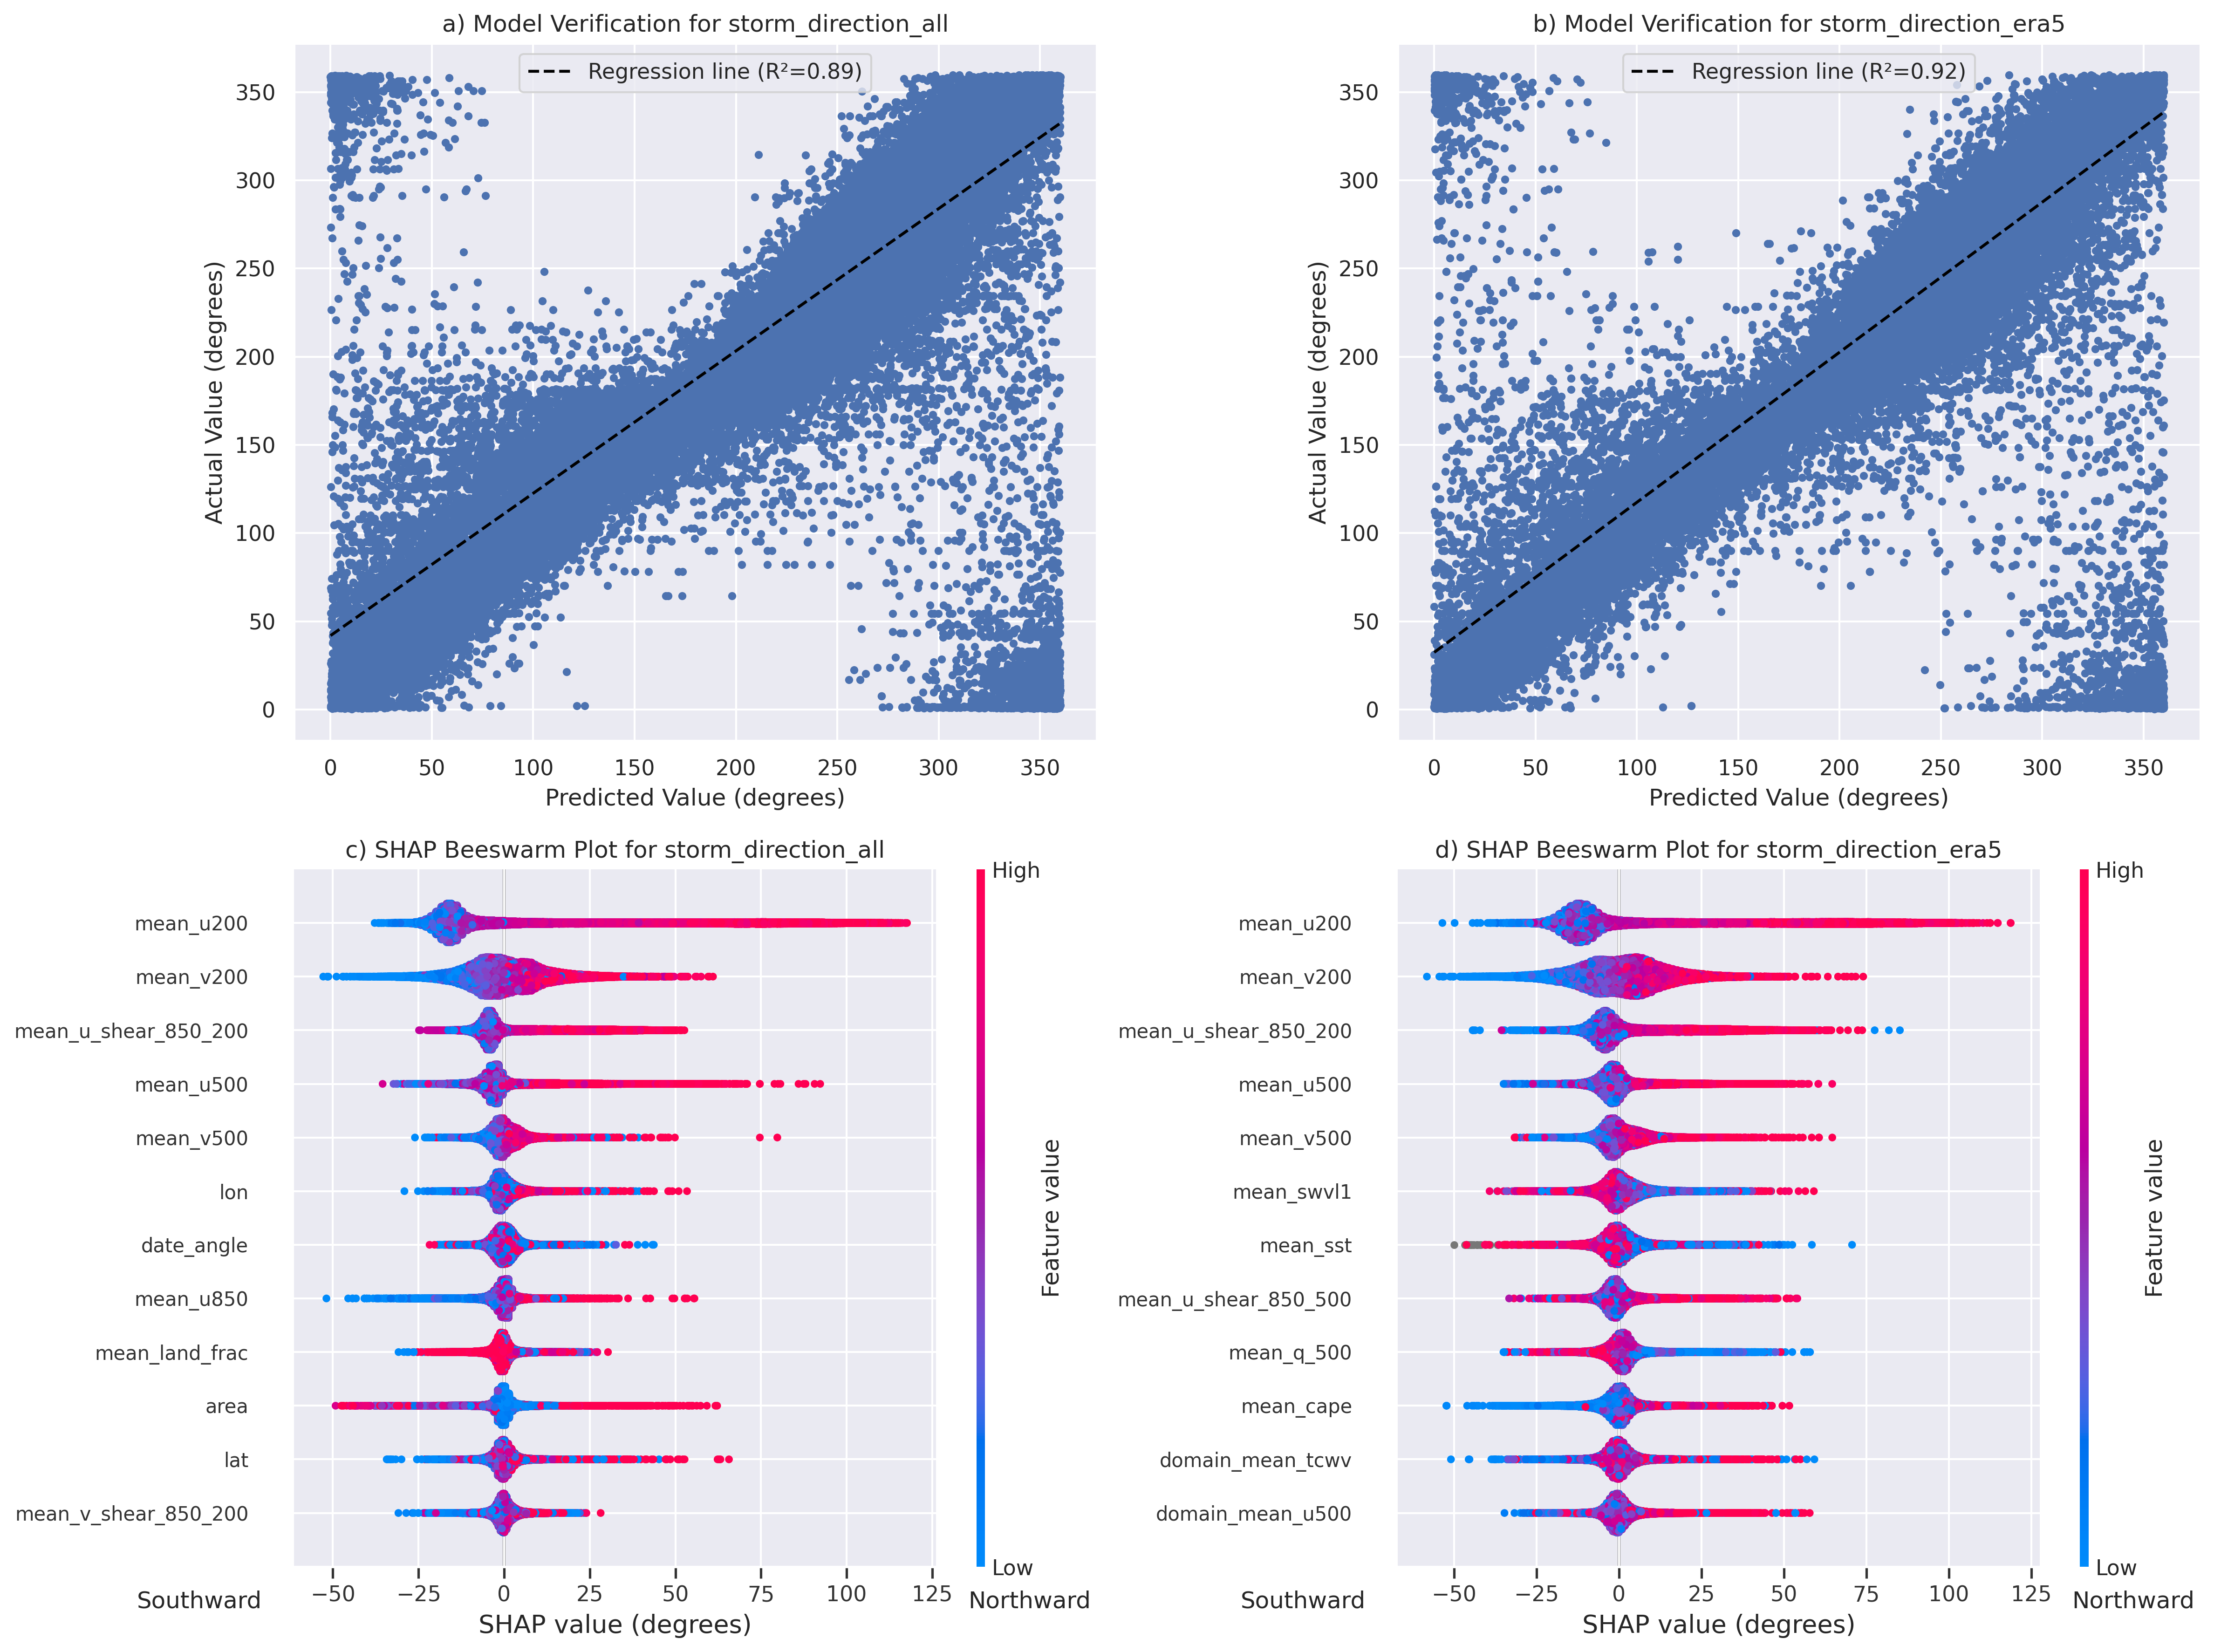
\includegraphics[width=\textwidth]{../figures/generated/experiments/storm_direction/storm_direction_summary.png}
    \caption{Comparison of performance and top features between the models trained on all features and ERA5 data only when predicting storm direction. Panels (a) and (b) show a comparison between predicted and actual values. The black dashed line shows the line of best fit and the resulting linear correlation coefficient between the actual and predicted values is displayed at the top of the plot. Panels (c) and (d) show top 12 predictors sorted by descending mean \acrshort{shap} value.}
    \label{fig:storm_direction_summary}
\end{figure}

High-level winds are by far the most important factors for predicting storm direction, as can be seen in panels (c) and (d) in Figure \ref{fig:storm_direction_summary}. Positive values of both meridional and zonal winds, southerly and westerly winds respectively, tend to shift the predicted storm direction northward and vice versa.

As shown in Figure \ref{fig:storm_direction_all_shap_mean_v850_map_by_month}, the effect of low-level meridional winds varies with location and time of year. From late spring to late summer, the influence is predominantly positive over the Somali coastal plains and negative over the northeastern Ethiopian (panels (i) through (r)), suggesting a convergence zone along the ridge line which extends north-eastward out from the Ethiopian Highlands. During the winter months, however, the \SI{850}{\hecto\pascal} meridional component is primarly northerly over the entire domain and resulting influence appears mostly negative, generally pushing storms southward (panels (a) through (h) and (s) through (x)).

\begin{figure}[ht]
    \centering
    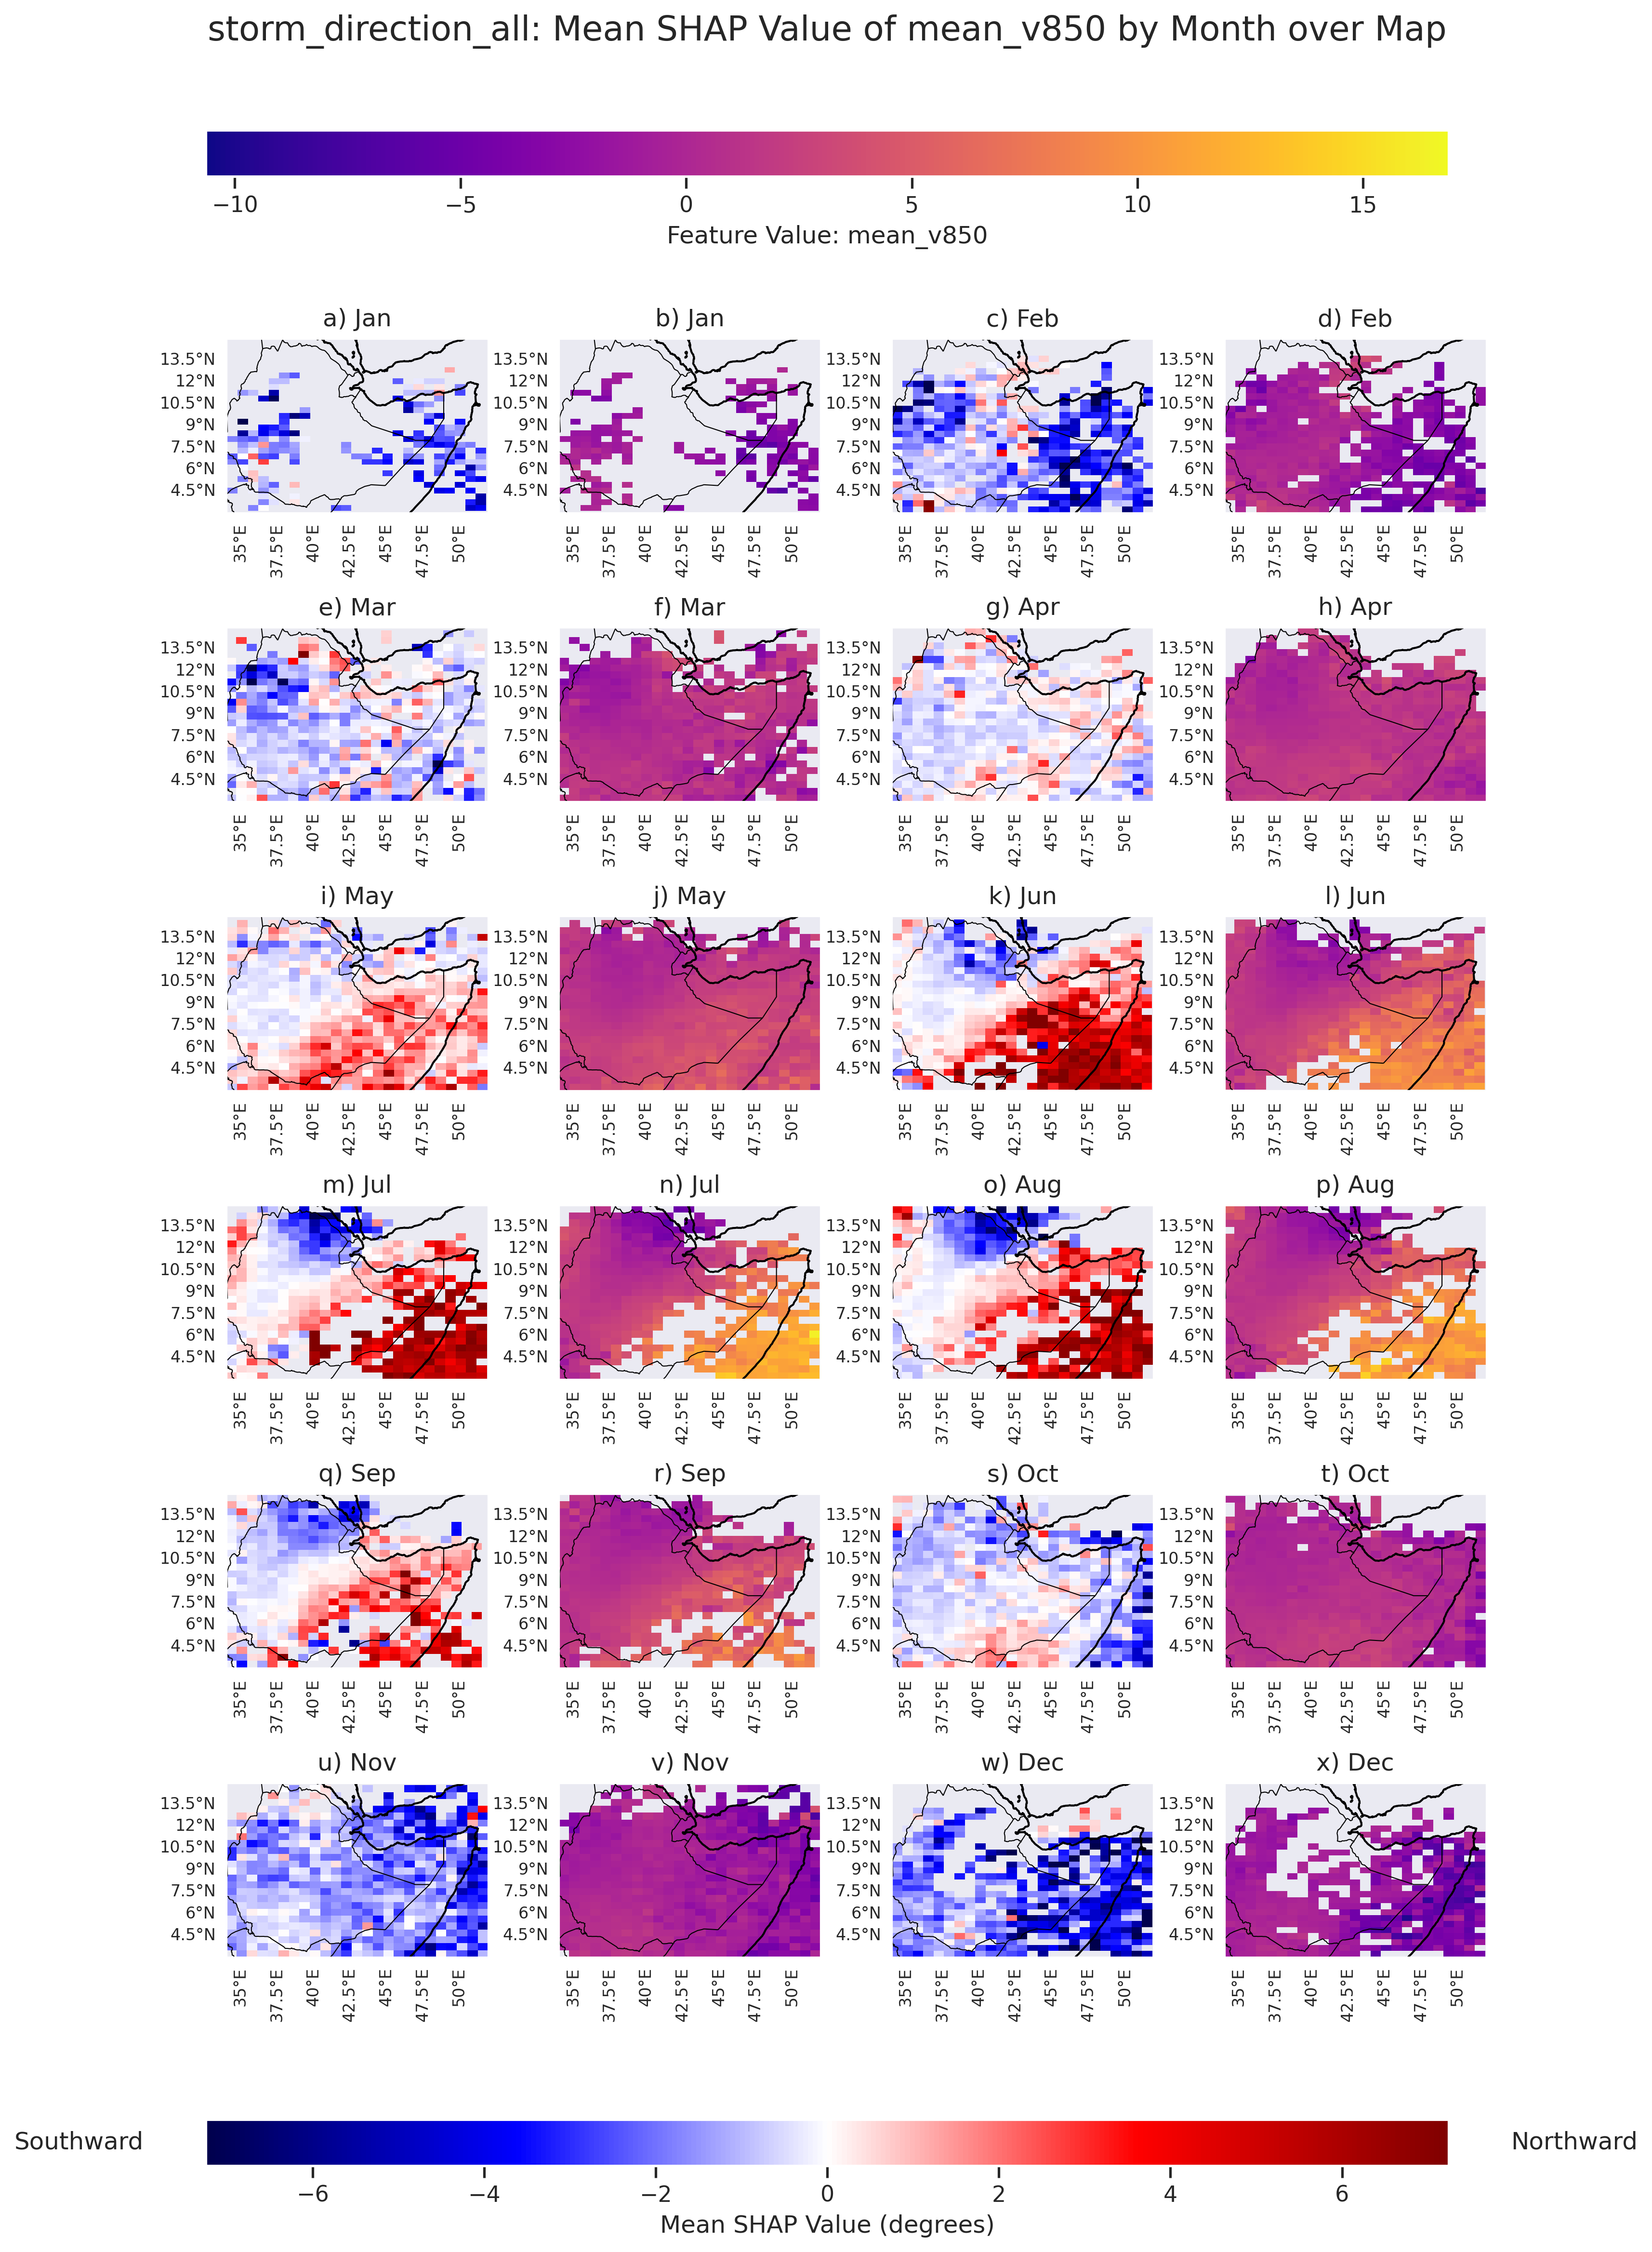
\includegraphics[width=\textwidth]{../figures/generated/experiments/storm_direction/geographic_corr/storm_direction_all_shap_mean_v850_map_by_month.png}
    \caption{Feature contribution of \SI{850}{\hecto\pascal} meridional wind over East Africa by month for storm direction prediction using all features. Plots are paired by month to compare mean \acrshort{shap} values (left) with feature values (right). For example, panel (a) shows mean \acrshort{shap} values for \SI{850}{\hecto\pascal} meridional wind for January measured in the units of the target variable (\unit{\kelvin}) and panel (b) shows the respective feature values for \SI{850}{\hecto\pascal} meridional wind for January in \unit{\meter\per\second}.}
    \label{fig:storm_direction_all_shap_mean_v850_map_by_month}
\end{figure}

\clearpage
\section{Predict Immediate Characteristics at an Observation}

These experiments aim to predict the immediate characteristics of a storm based on its current observation and Table \ref{tab:obs_experiment_results} shows performance metrics of the models. 

Unfortunately, \acrshort{xgb} struggled to accurately predict the next direction and distance of the storm, as indicated by the \acrshort{rmse} values being only slightly lower than the standard deviation of the target variable. For storm direction, the \acrshort{rmse} was $62.3535$ and $62.4498$ for all features and \acrshort{era5} features respectively, compared to a standard deviation of $72.9832$. Similarly, for storm distance, the \acrshort{rmse} was $12.0634$ and $12.6901$ for all features and \acrshort{era5} features respectively, compared to a standard deviation of $13.1260$. As such, no further explainability analysis will be conducted on those experiments. However, possible reasons for this poor performance and future directions for improvement are discussed in Section \ref{sec:results-propagation}.

Models predicting intensification and precipitation did show more promise, with lower \acrshort{rmse} values compared to their corresponding target standard deviations. For intensification, the \acrshort{rmse} was $2.8149$ and $3.0828$ for all features and \acrshort{era5} features respectively, compared to a standard deviation of $4.4840$. For precipitation, the \acrshort{rmse} was $0.0488$ and $0.0851$ for all features and \acrshort{era5} features respectively, compared to a standard deviation of $0.1835$.

Contrary to the results for predicting storm maximum intensity, the performance of the models using all features was better than those using only \acrshort{era5} features for both intensification and precipitation. This suggests that the non-meteorological features provide valuable information for these tasks.

\begin{table}[h!]
\centering
\caption{Experimental results for immediate characteristic at observation prediction}
\label{tab:obs_experiment_results}
\begin{tabular}{lccc}
\hline
\textbf{Experiment} & \textbf{Test RMSE} & \textbf{Target Std} & \textbf{Units} \\
\hline
Intensification All & 2.8149  & \multirow{2}{*}{4.4840}  & \multirow{2}{*}{\unit{\kelvin}} \\
Intensification \acrshort{era5} & 3.0828  & &  \\ \hline
Direction All & 62.3535 & \multirow{2}{*}{72.9832} & \multirow{2}{*}{\unit{\degree}} \\
Direction \acrshort{era5} & 62.4498 & & \\ \hline
Distance All & 12.0634 & \multirow{2}{*}{13.1260} & \multirow{2}{*}{\unit{\km}} \\
Distance \acrshort{era5} & 12.6901 & & \\ \hline
Precipitation All & 0.0488  & \multirow{2}{*}{0.1835}  & \multirow{2}{*}{\unit{\milli\meter}} \\
Precipitation \acrshort{era5} & 0.0851  & & \\
\hline
\end{tabular}
\end{table}

\clearpage
\subsection{Intensification}
\label{sec:results-intensification}

Although the \acrshort{rmse} of the models are acceptable, it is evident that the models from both feature sets generally tend to underpredict intensification and weakening. This behaviour can be seen in the clustering of points below the regression line in both panels (a) and (b) in Figure \ref{fig:obs_intensification_summary}. These are instances where the actual rate of intensification is higher than predicted. 

It should be noted that in panel (b), there are a significant number of points where the \acrshort{era5}-features-only model predicted no intensification (i.e., a rate of intensification of zero) when the actual values are both positive and negative. The same behaviour can not be observed for the all features model in panel (a). From these plots and analysis below, it is not immediately clear why this discrepancy exists and further investigation is warranted.

\begin{figure}[ht]
    \centering
    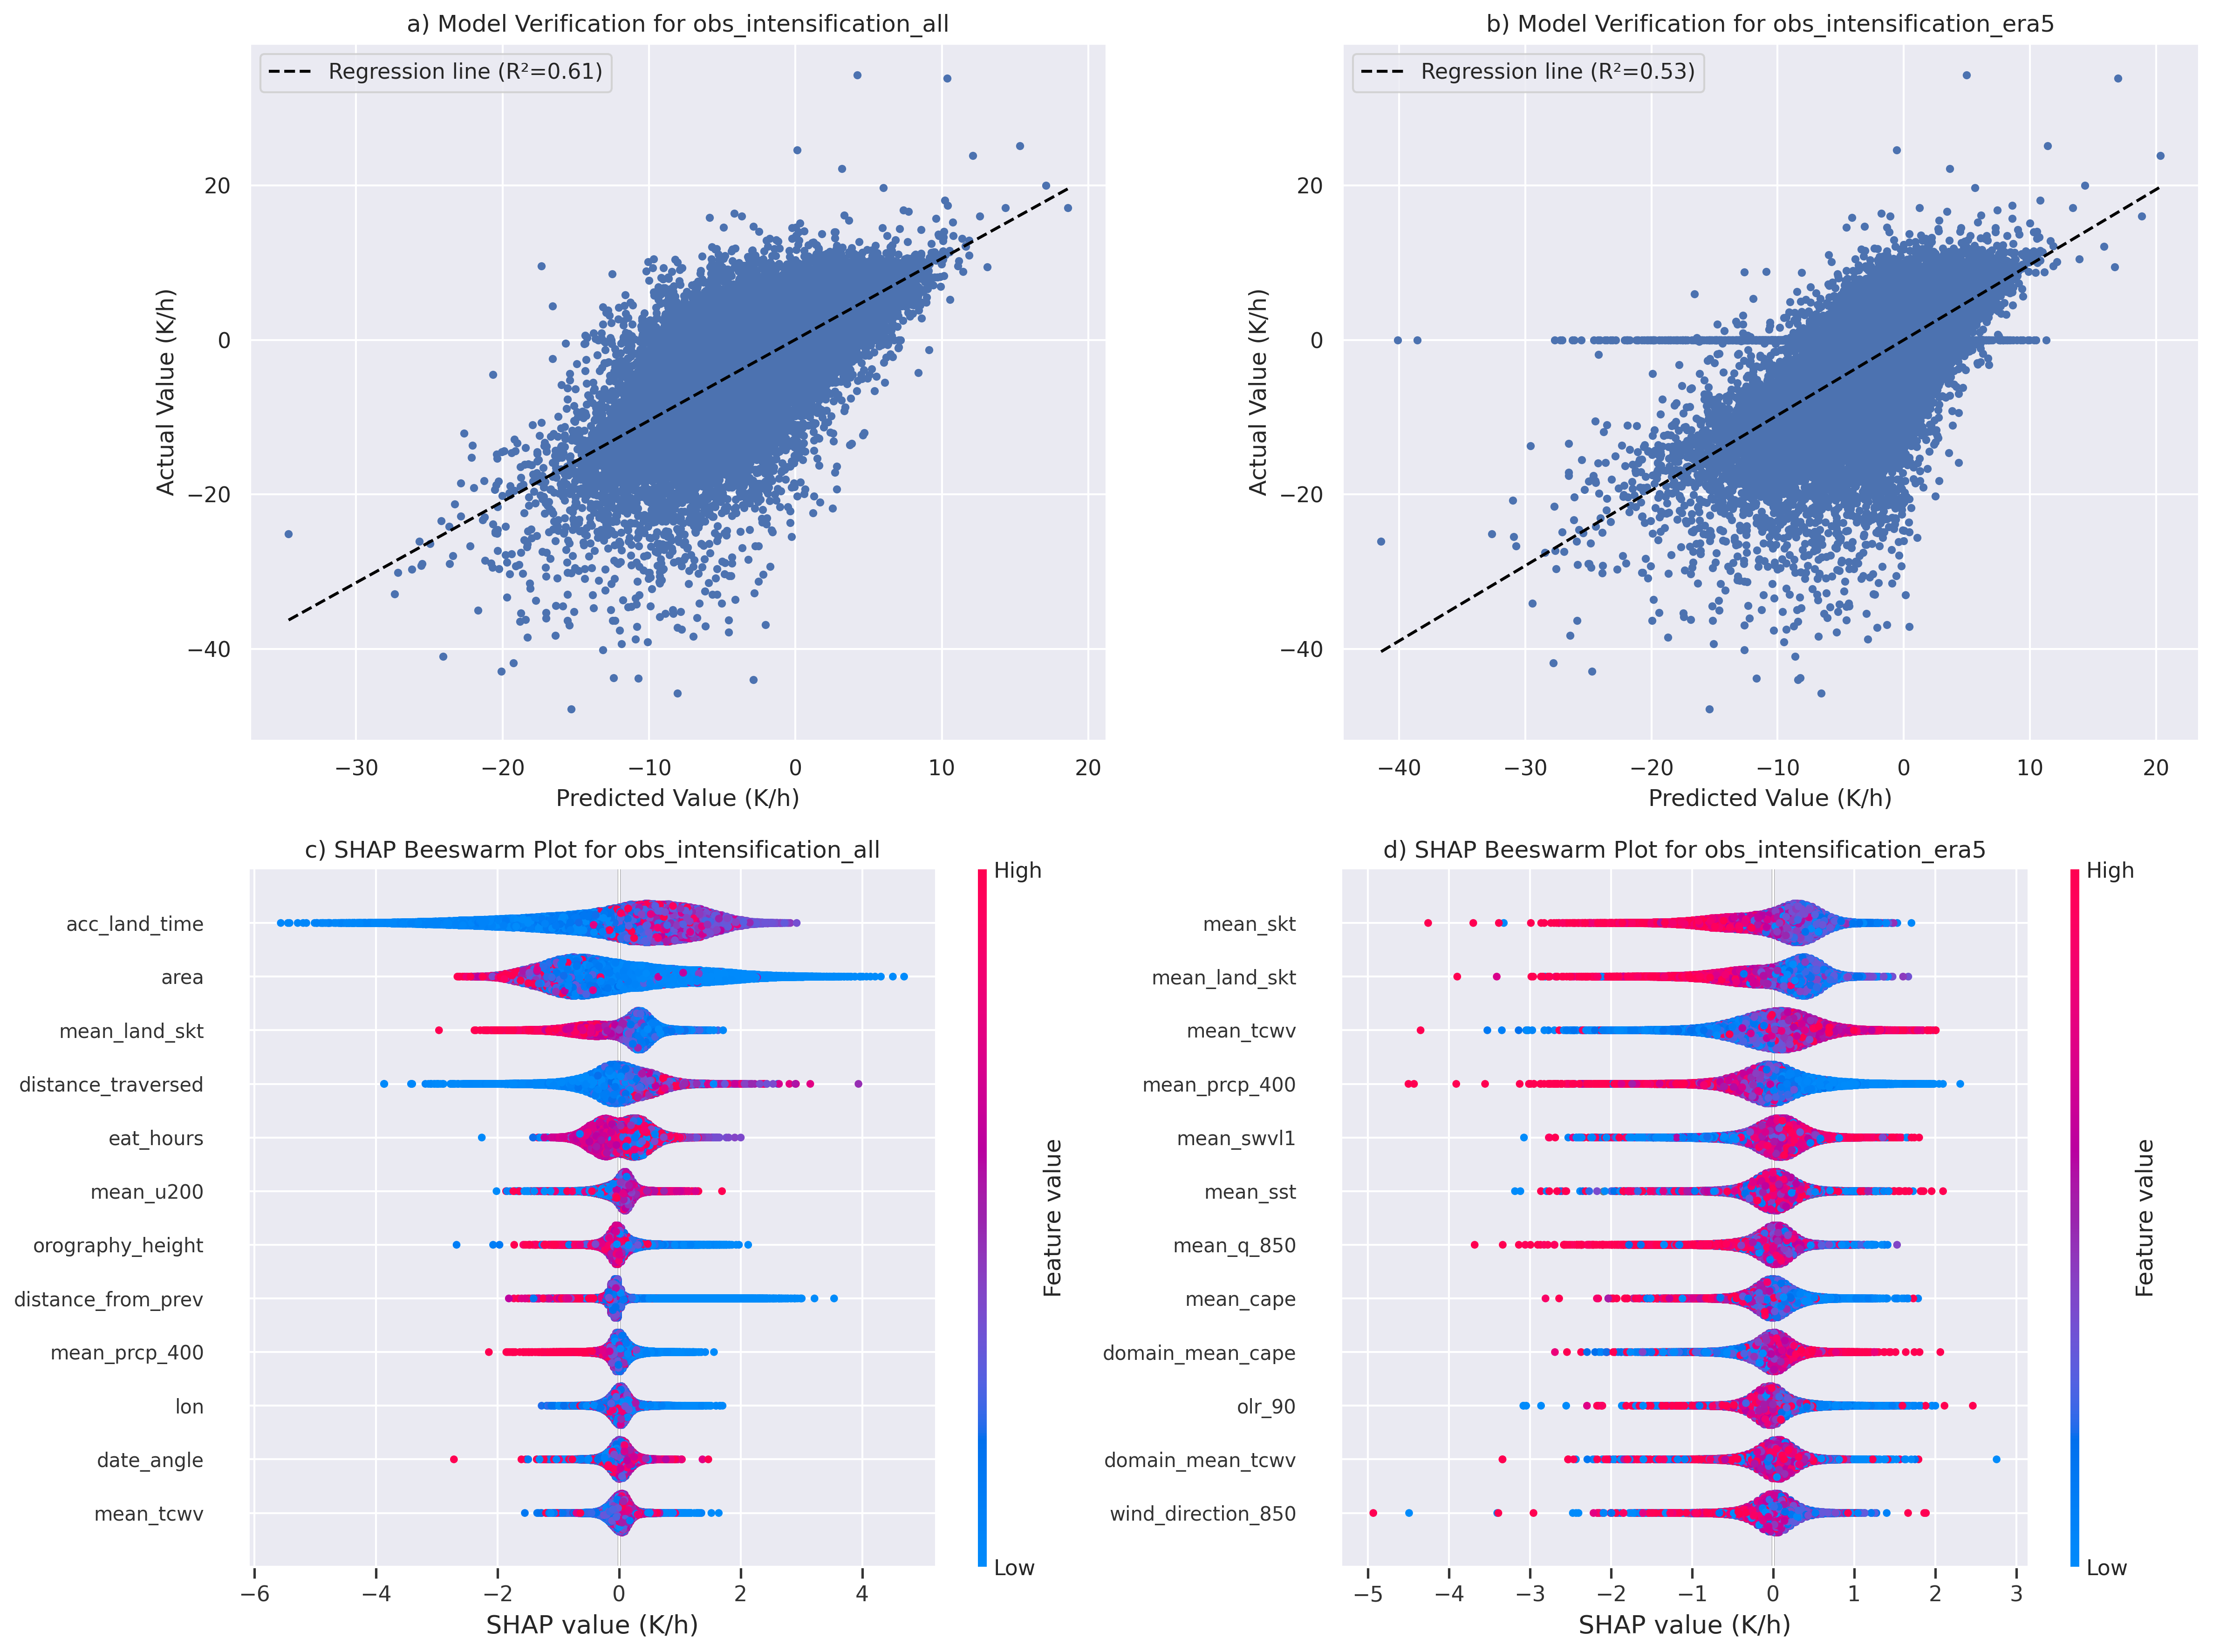
\includegraphics[width=\textwidth]{../figures/generated/experiments/obs_intensification/obs_intensification_summary.png}
    \caption{Comparison of performance and top features between the models trained on all features and ERA5 data only when predicting storm intensification. Panels (a) and (b) show a comparison between predicted and actual values. The black dashed line shows the line of best fit and the resulting linear correlation coefficient between the actual and predicted values is displayed at the top of the plot. Panels (c) and (d) show top 12 predictors sorted by descending mean \acrshort{shap} value.}
    \label{fig:obs_intensification_summary}
\end{figure}

As for the feature contributions (Figure \ref{fig:obs_intensification_summary} panels (c) and (d)), surface characteristics seem to be especially important. In the \acrshort{era5} model (panel (d)), land skin and sea surface temperature both appear in the top ten features. Across both models, high land skin temperature contributes to storm intensification. Related is the high importance of soil moisture, but the specific nature of its contribution is less clear as both high and low feature values can accelerate or decelerate intensification. Lastly, storms also tend to intensify more when they spend longer periods over the ocean. This is consistent with the known role of heat flux and moisture availability over the ocean in sustaining and intensifying convective systems \citep{Klein2021,Sud1998,Abbott2025}.

In contrast to storm maximum intensity, \acrshort{cape} is less important for predicting intensification. The contributions of mean \acrshort{cape} and domain mean \acrshort{cape} notably have opposite effects on intensification. One interpretation of this result is that localised, anomalous instability may play a more significant role than broader atmospheric conditions, but more analysis is required to confirm the relationship.

\acrfull{tcwv}'s feature contribution for the model trained on only \acrshort{era5} data is unexpected based on the theoretical relationship. The fact that it does has strong contributions to both models is expected \citep{Li2023,Muetzelfeldt2025,Klein2020}. However, the relationship between its contribution and the feature value should be reversed. According to the beeswarm plot (panel (d) in Figure \ref{fig:obs_intensification_summary}), higher values of mean \acrshort{tcwv} tend to slow intensification whereas low values accelerate it.

The spatial and temporal distribution of mean \acrshort{tcwv} values and their corresponding SHAP values in Figure \ref{fig:obs_intensification_era5_shap_mean_tcwv_map_by_hour} sheds light on what might be driving this unexpected relationship. As can be seen, low values of mean \acrshort{tcwv} are generally concentrated over the Ethiopian Highlands and surrounding elevated terrain. This relationship is confirmed in the correlation heatmap in Appendix \insertref{appendix corr heatmap} where mean \acrshort{tcwv} has a correlation coefficient of -0.59 with elevation and visually in Figure \insertref{fig:tcwv\_mean\_by\_loc}.

One interpretation of this result could be that orographic lifting causes moist air to rise and condense, leading to precipitation and thus lower \acrshort{tcwv} values. The storms are then more likely to intensify when they are situated over or near elevated terrain, where orographic effects can enhance convection. This hypothesis may be bolstered by subplots g) and i) in Figure \ref{fig:obs_intensification_era5_shap_mean_tcwv_map_by_hour} which show enhanced intensification over the highlands in the late afternoon, as is consistent with the diurnal cycle of orographic lifting \citep{Colle2015,Negash2024,Zardi2013}.

Alternately, the counter-intuitive relationship may be a result of excluding orographic variables from the model. Indeed, the beeswarm plot for feature contribution of the model trained on all features ((c) in Figure \ref{fig:obs_intensification_summary}) shows that high elevation has a strong positive contribution to intensification. Farther down the in same plot, the feature value of mean \acrshort{tcwv} shows no clear pattern for slowing or accelerating intensification. Thus, the behaviour displayed in Figure \ref{fig:obs_intensification_era5_shap_mean_tcwv_map_by_hour} may be an artifact of the dataset, where storms over the Ethiopian Highlands tend to form during the early afternoon and intensify rapidly. However, orographic elevation does not show this same relationship for storm max intensity, further complicating the interpretation.

Notwithstanding, perhaps the most important interpretation of these results is that a cautious and deliberate approach must be undertaken when using \acrshort{ml} models to study complex atmospheric phenomena. While these models are powerful and clearly capable of capturing complex patterns, their accuracy may engender a false sense of confidence, especially if they are not carefully validated against domain knowledge. Therefore, it is crucial to combine \acrshort{ml} with meteorological expertise to ensure robust and trustworthy implementations.

\begin{figure}[ht]
    \centering
    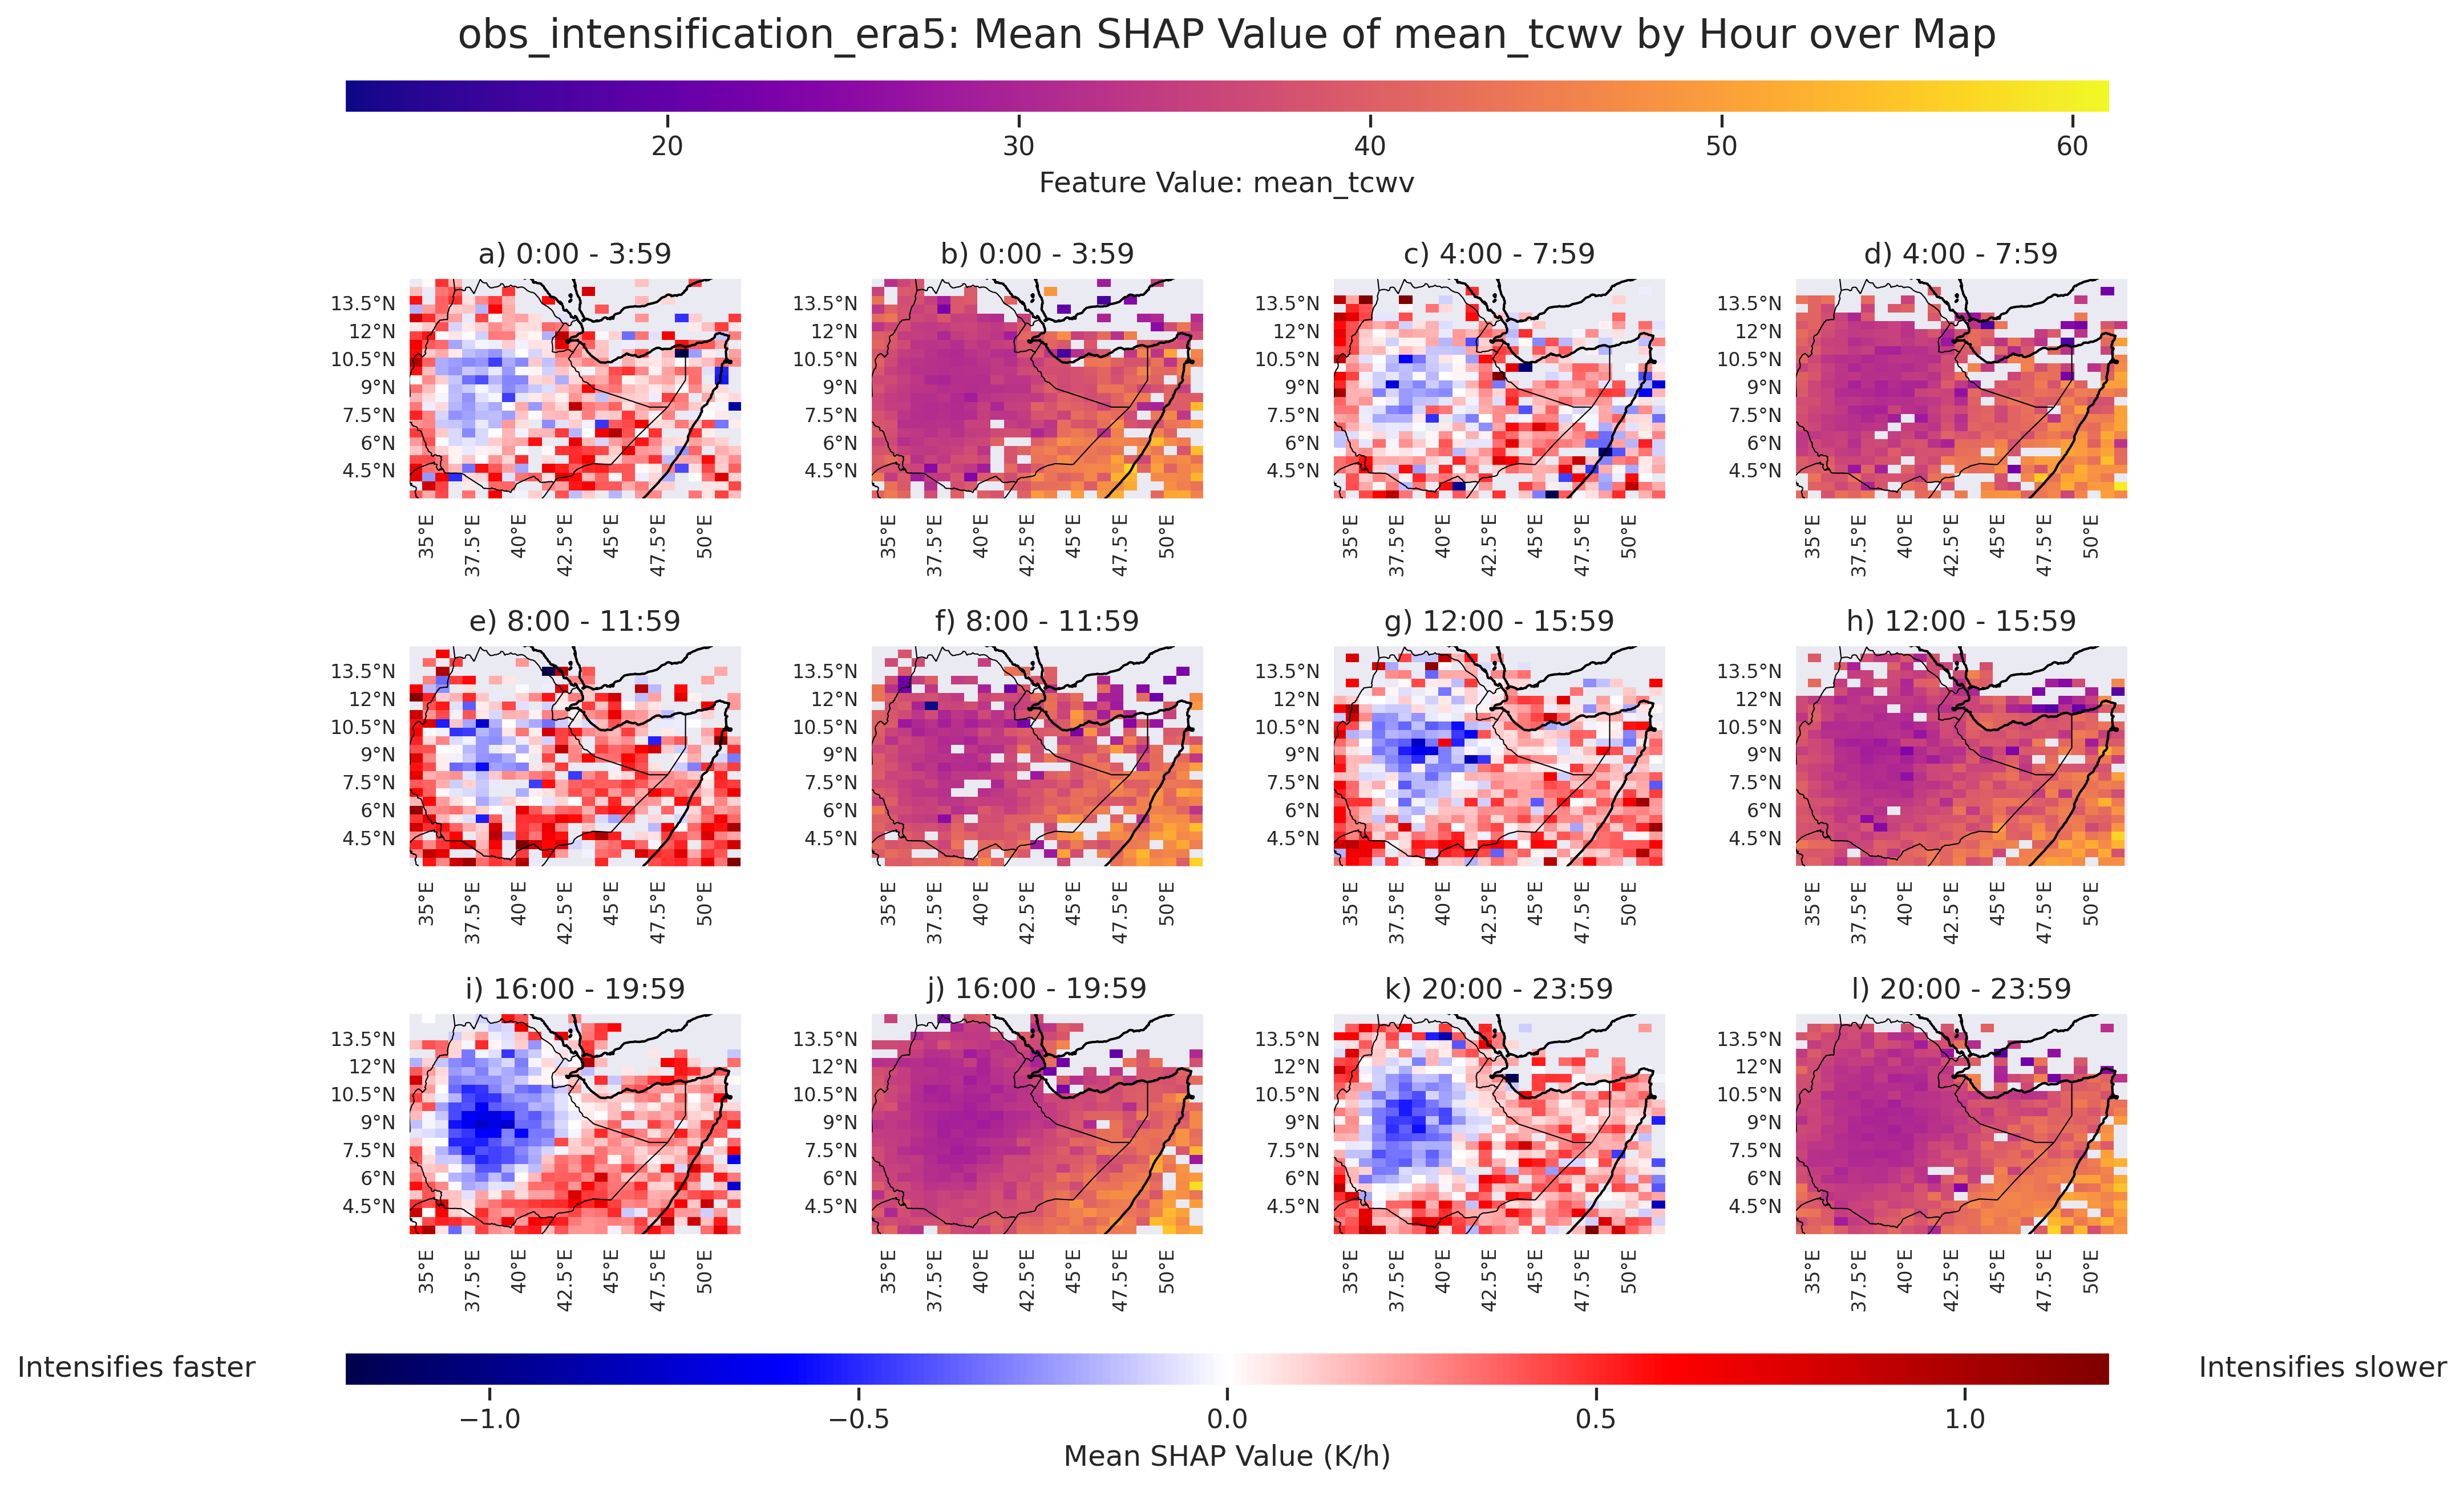
\includegraphics[width=\textwidth]{../figures/generated/experiments/obs_intensification/geographic_corr/obs_intensification_era5_shap_mean_tcwv_map_by_hour.png}
    \caption{Feature contribution of \acrshort{tcwv} over East Africa by hour for rate of intensification prediction using \acrshort{era5} features. Plots are paired by hour to compare mean \acrshort{shap} values (left) with feature values (right). For example, panel (a) shows mean \acrshort{shap} values for mean \acrshort{tcwv} for the hours 00:00 - 03:59 \acrshort{eat} measured in the units of the target variable (\unit{\kelvin\per\hour}) and panel (b) shows the respective feature values for mean \acrshort{tcwv} for the hours 00:00 - 03:59 \acrshort{eat} in \unit{\kilogram\per\meter\squared}.}
    \label{fig:obs_intensification_era5_shap_mean_tcwv_map_by_hour}
\end{figure}

Lastly for the intensification experiment, Figure \ref{fig:obs_intensification_sst_skt_by_hour} shows the temporal variability of the mean SHAP values for \acrfull{sst} (panel (a)) and land skin temperature (panel (b)). Here we might postulate that the slight offset between the hours where each variable contributes most strongly to intensification corresponds to the diurnal cycle of the heating of the Earth surface, with land skin temperature peaking during midday and \acrshort{sst} lagging by a few hours. This analysis could be used to calibrate threshold values at which these variables begin to contribute to \acrshort{mcs} intensification for convection parametrisation schemes. In addition to threshold values, the relative importance of these two variables could also be used to inform the weighting of land versus ocean surface fluxes as well as the magnitude of the effect based on the relationship between the change in \acrshort{shap} value per unit change in surface temperature.

\begin{figure}[ht]
    \centering
    \begin{subfigure}[t]{\textwidth}
        \centering
        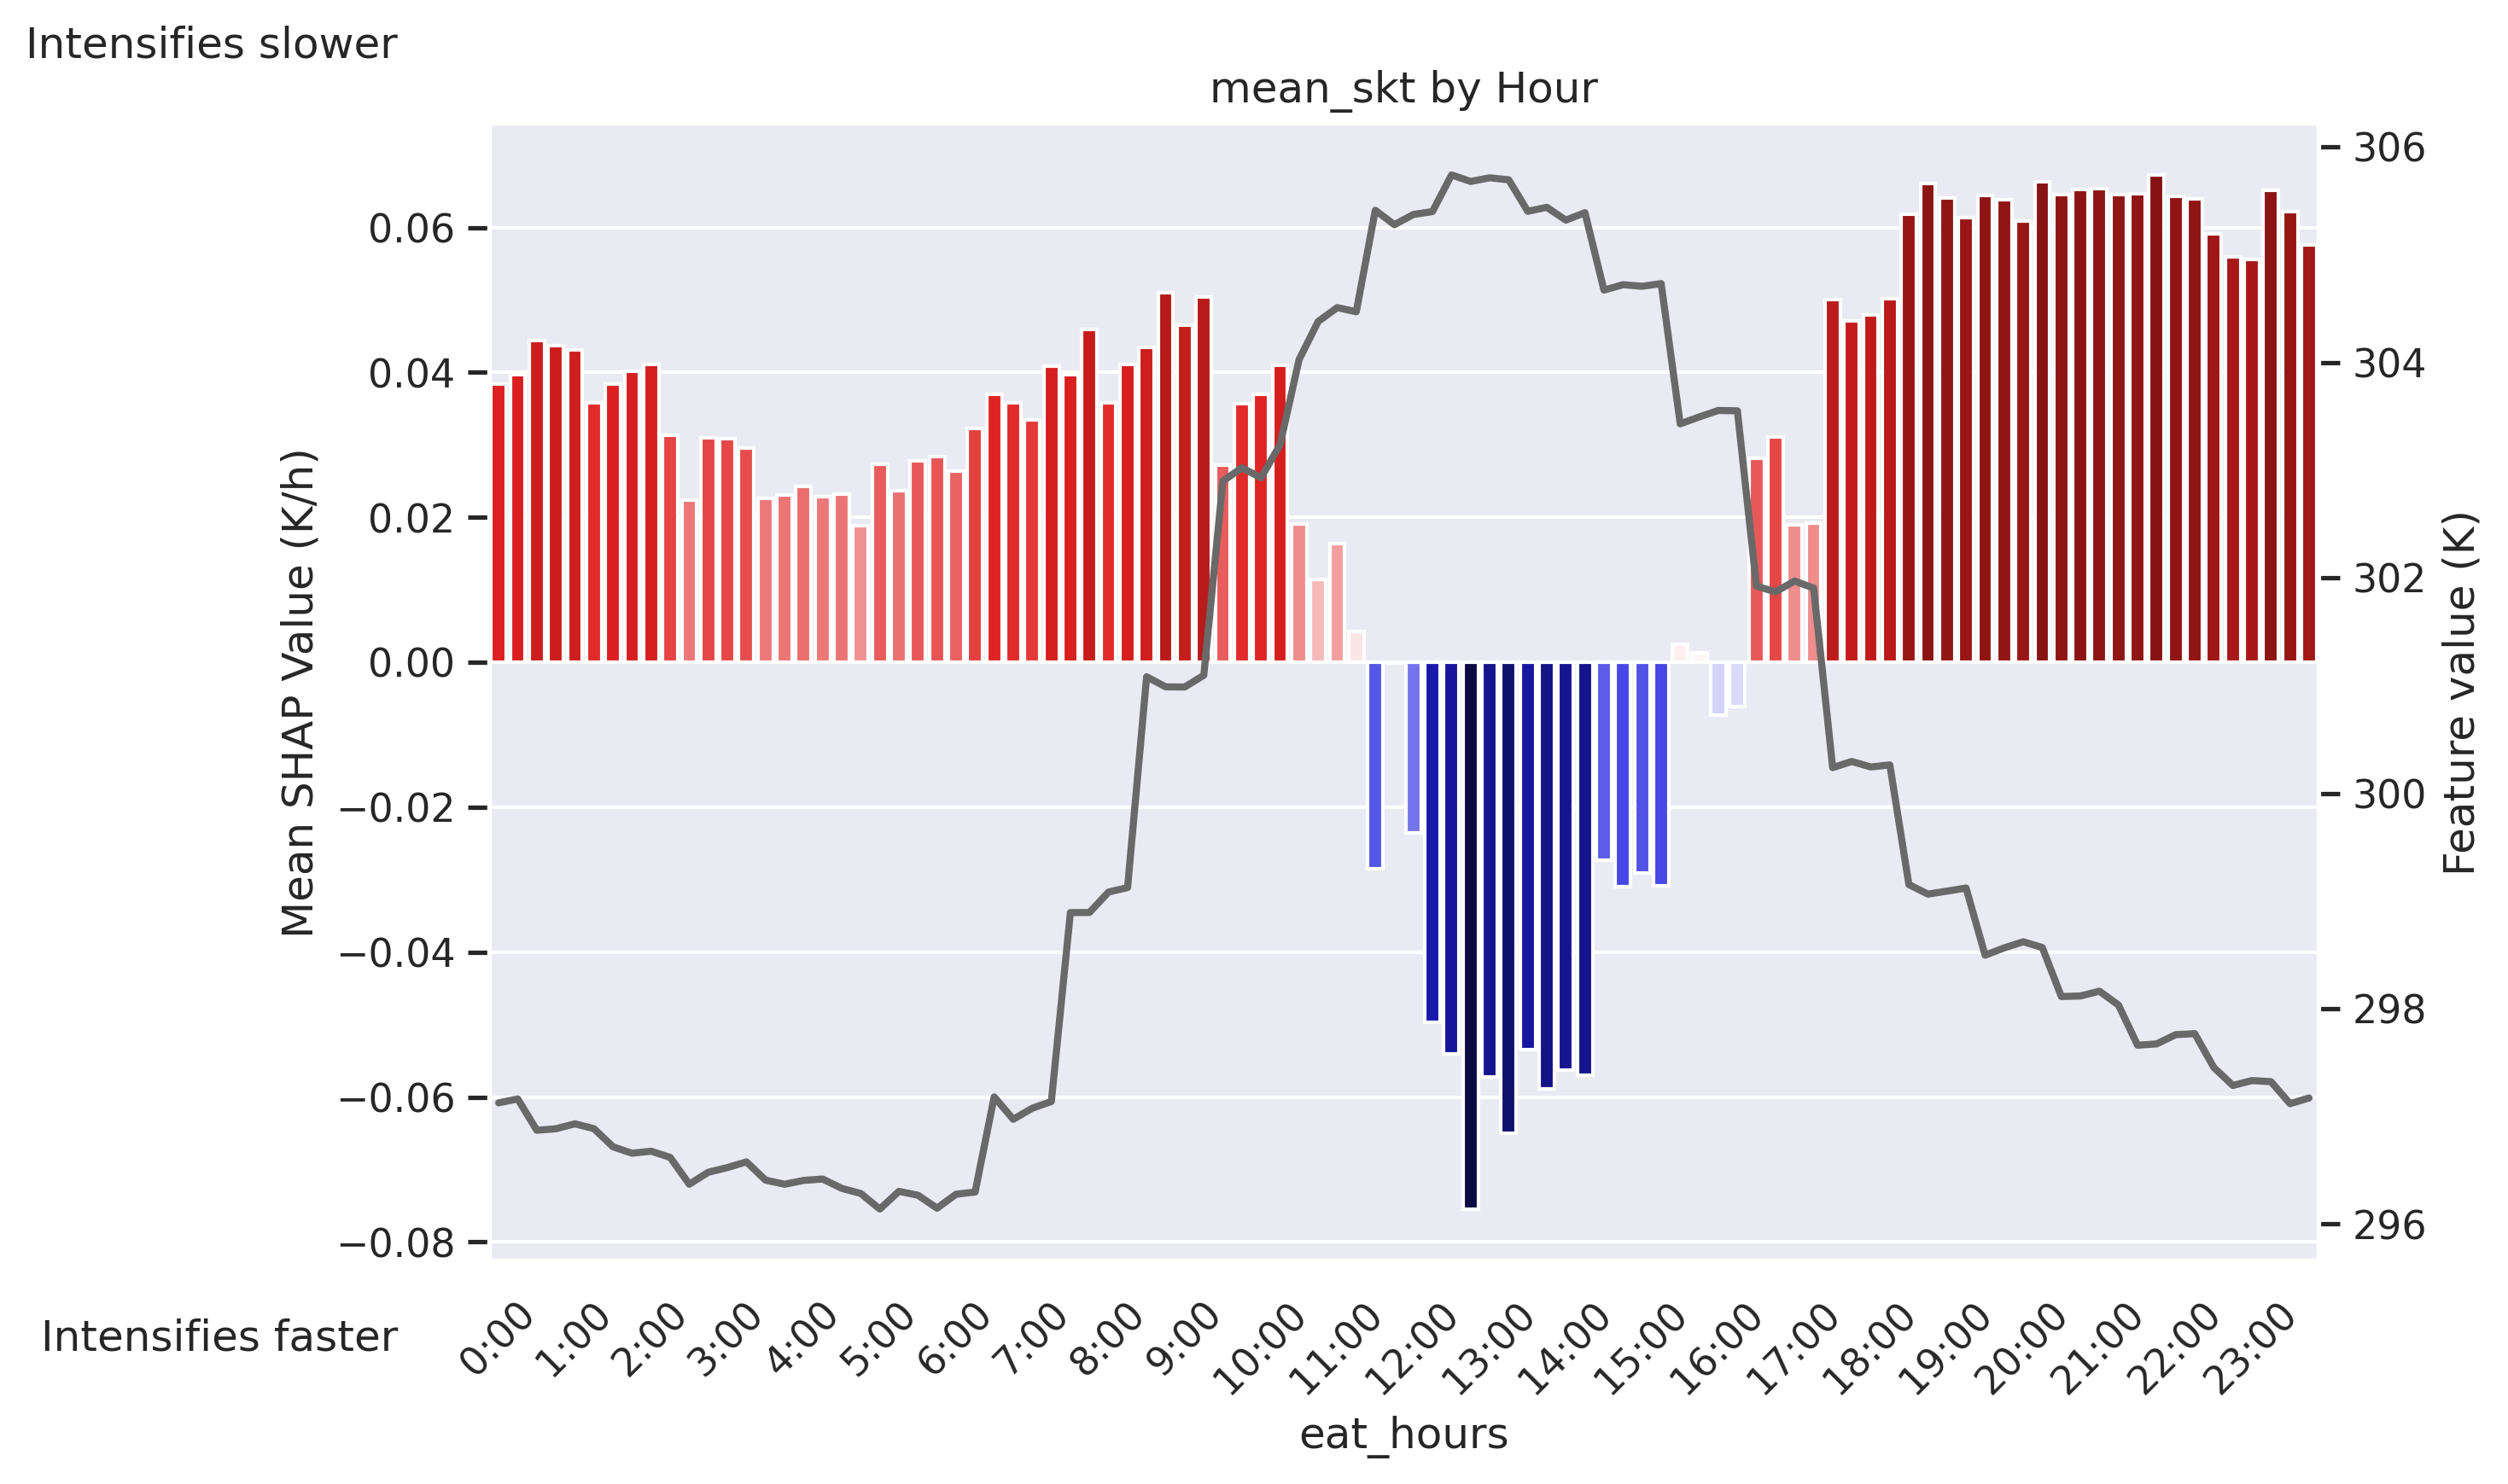
\includegraphics[width=\textwidth]{../figures/generated/experiments/obs_intensification/temporal_corr/obs_intensification_all_shap_mean_skt_by_hour.png}
        \caption{Temporal variability of SHAP values for mean land skin temperature by hour for the intensification model with all features.}
        \label{fig:obs_intensification_all_shap_mean_skt_by_hour}
    \end{subfigure}
    \vspace{1em}
    \begin{subfigure}[t]{\textwidth}
        \centering
        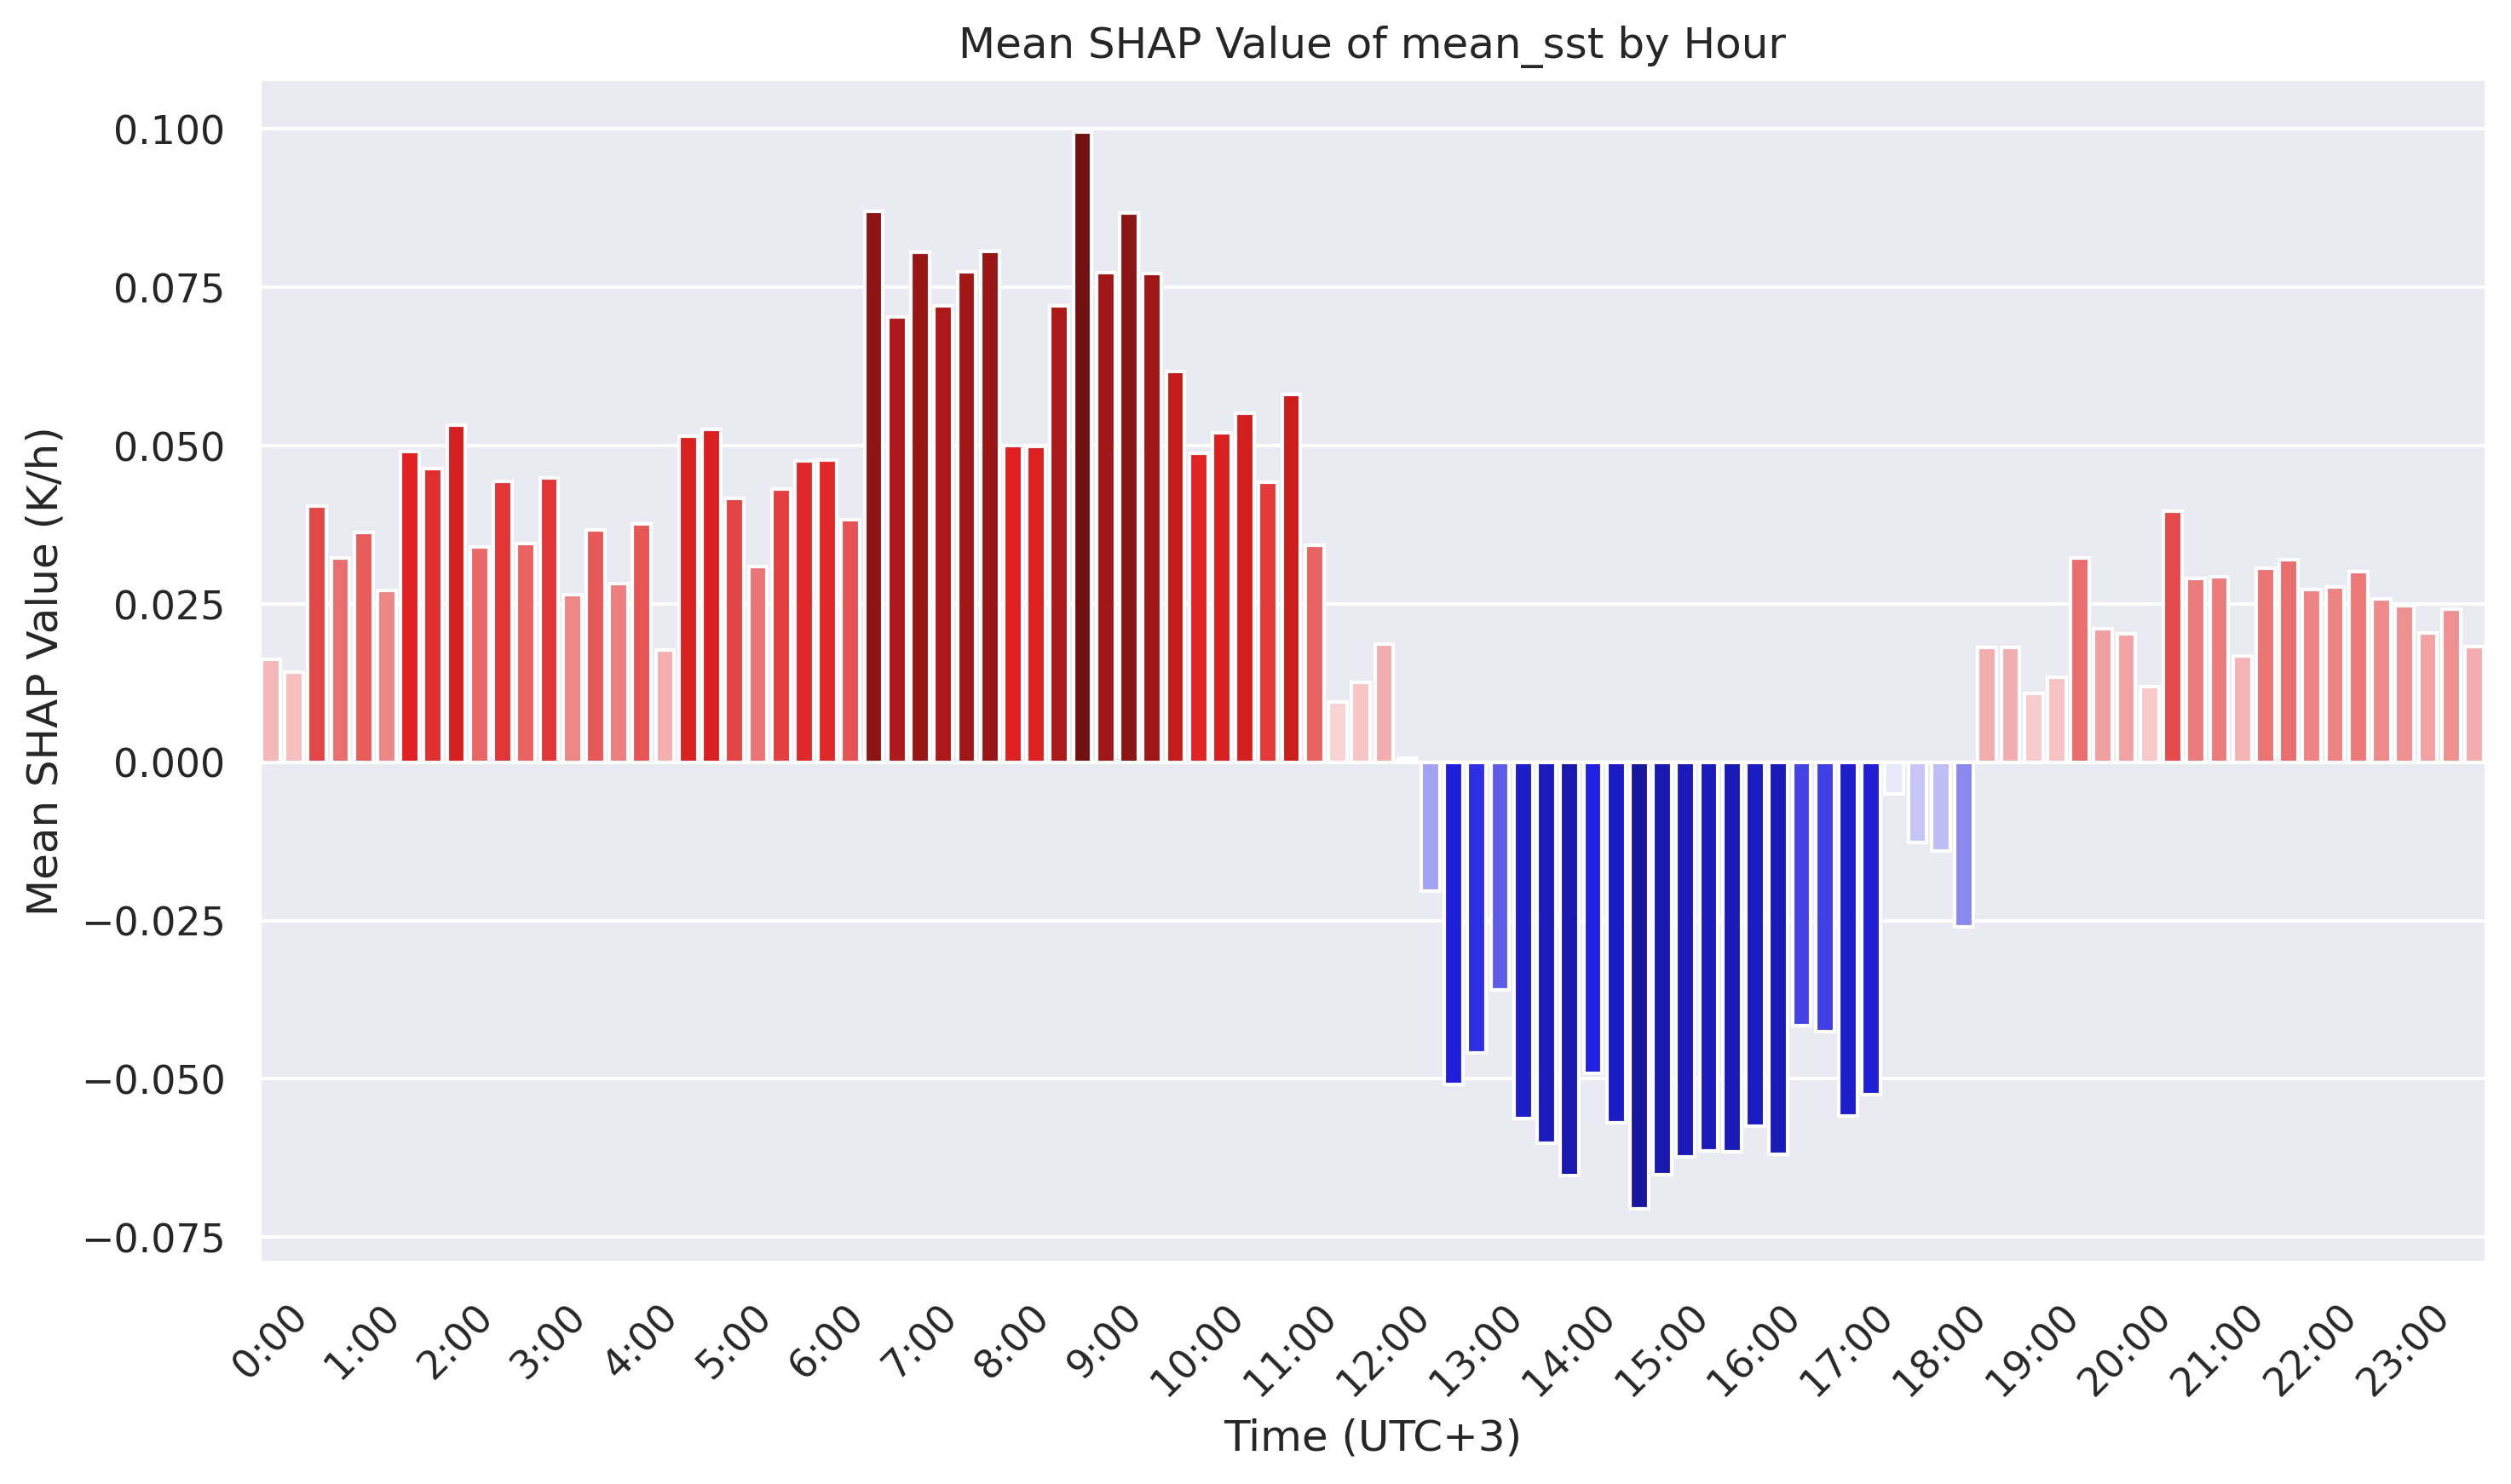
\includegraphics[width=\textwidth]{../figures/generated/experiments/obs_intensification/temporal_corr/obs_intensification_era5_shap_mean_sst_by_hour.png}
        \caption{Temporal variability of SHAP values for mean sea surface temperature by hour for the intensification model with only \acrshort{era5} features.}
        \label{fig:obs_intensification_era5_shap_mean_sst_by_hour}
    \end{subfigure}
    \caption{Comparison of mean \acrshort{shap} value for \acrshort{sst} and land skin temperature by hour for the intensification models.}
    \label{fig:obs_intensification_sst_skt_by_hour}
\end{figure}

\subsection{Propagation}
\label{sec:results-propagation}

As shown in Tables \ref{tab:storm_direction_results} and \ref{tab:obs_experiment_results} respectively, storm direction models perform well, but models predicting the direction and distance to the next observation perform poorly. This could be due to several factors. The calculation of the next direction relies on the centroid of the storm provided by \cite{Hill2023}. For \acrshortpl{mcs}, the centroid might be weakly defined as the storm structure does not often have a clear centre of circulation compared to other systems like tropical cyclones. For example, squall lines are linear features and the centroid location outputted by the tracking algorithm may vary significantly between each time step based on the shape and orientation of the line. This would lead to particularly noisy data. To mitigate this, future work should investigate smoothing the centroid trajectory to reduce noise and improve the reliability of movement estimates.

For direction specifically, although modifications were made to the \acrshort{rmse} function used to train and evaluate the models to account for the nature of circular data, this still appeared to limit the capabilities of the models. Alternative approaches, such as using categorical representations of the compass bearing (i.e., N, NNE, NE, etc.) or transforming the degrees using sine and cosine functions may prove to be helpful for the models to effectively predict direction. Although the categorical approach would be more intuitive, it would sacrifice granularity. Sine and cosine transformations would likely be the optimal choice as they allow for continuous predictions. However, this would require either a multiple-output model or multiple models, thus increasing the complexity of the training process and explainability analysis. An analogue for this approach would be to use the zonal and meridional speed vectors instead of distance and direction as was done in \cite{Hunt2024}. Across all these methods, the same challenges of a weakly-defined storm centroid would still apply, and an investigation into the stability of the storm tracks would be necessary.

\clearpage
\subsection{Precipitation}

Unlike the other experiments, there is a meaningful discrepancy in performance between the \acrshort{era5}-only feature set and all features. The \acrshort{rmse} for the model trained on all features was $0.0488$, almost half that of the \acrshort{era5}-only features model with $0.0851$ \acrshort{rmse}. This would indicate that the included meteorological variables are insufficient to fully capture the factors influencing precipitation. This is further supported by the top feature for the \acrshort{era5}-only model being mean land skin temperature (panel (d) in Figure \ref{fig:obs_precipitation_summary}), a feature that is highly correlated with time of day as depicted in Figure \ref{fig:obs_precipitation_era5_shap_mean_land_skt_by_hour}. Although included in the all features model, \acrfull{bt} does not appear among the top features. However, \acrfull{olr}, a known proxy for cloud cover, is an important feature. This may indicate that overall cloud cover is more important than storm intensity for predicting precipitation. As in the previous experiment, mean \acrshort{cape} and domain mean \acrshort{cape} have opposite contributions to precipitation.

\begin{figure}[ht]
    \centering
    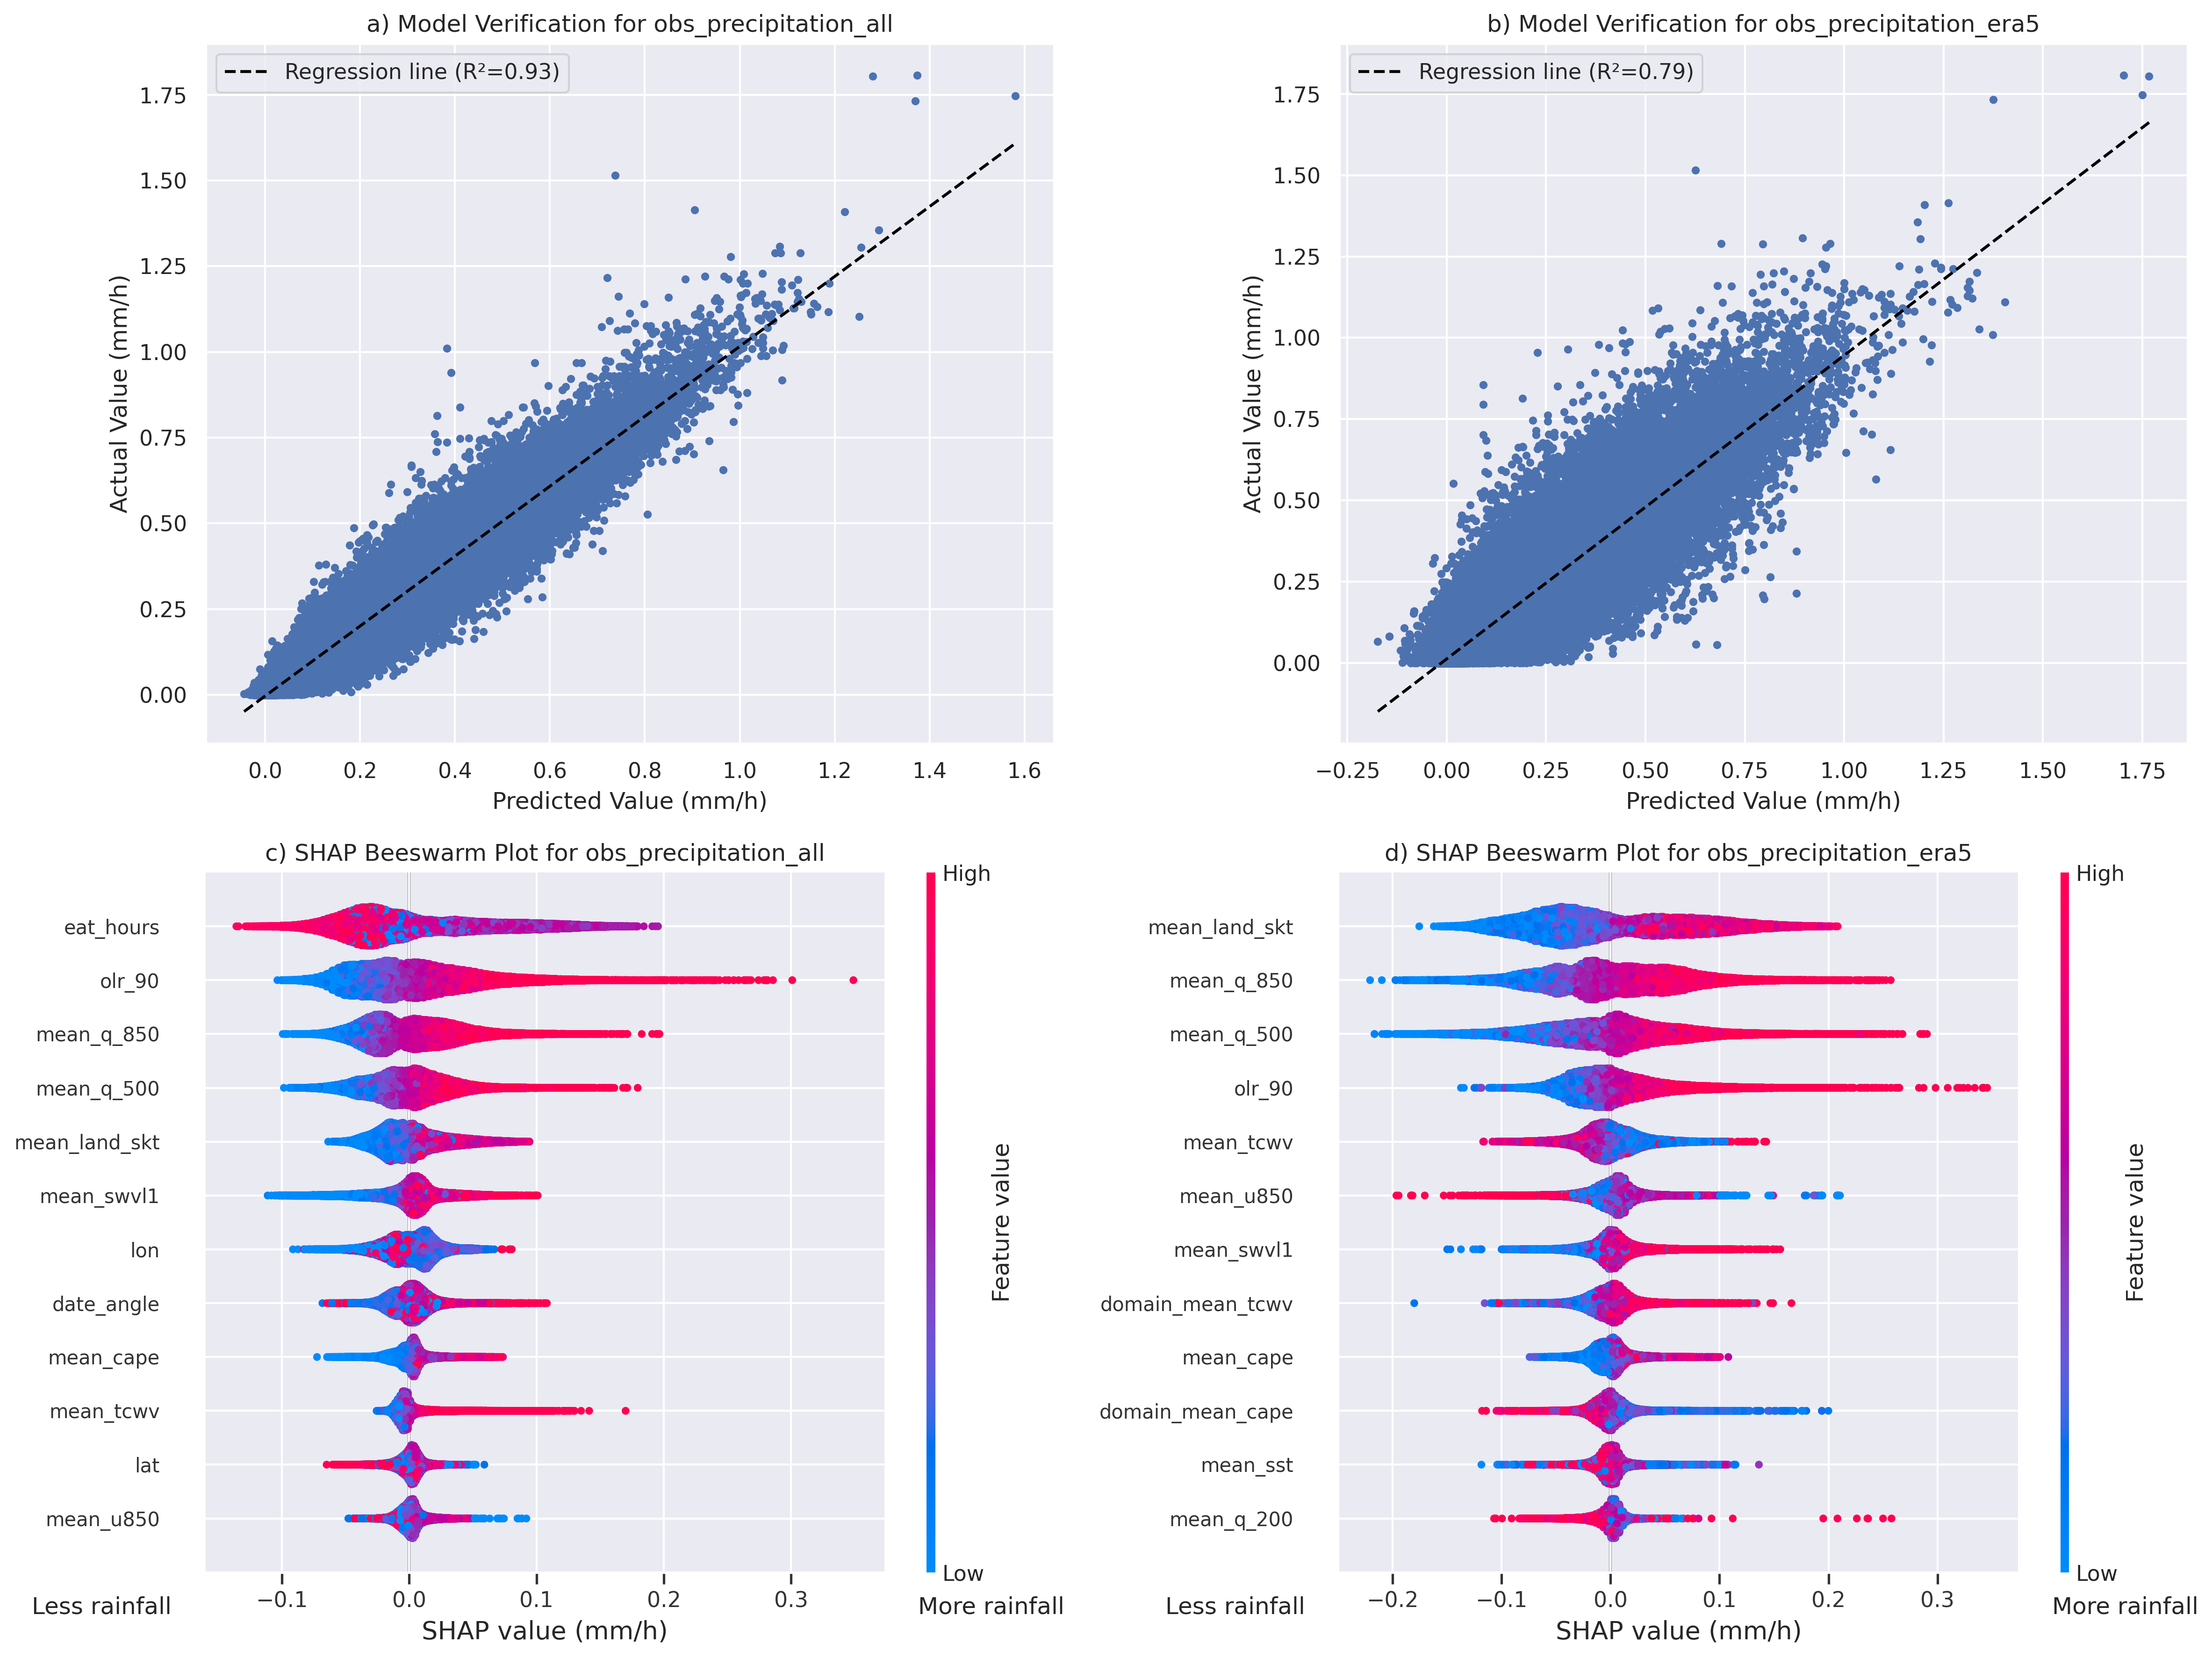
\includegraphics[width=\textwidth]{../figures/generated/experiments/obs_precipitation/obs_precipitation_summary.png}
    \caption{Comparison of performance and top features between the models trained on all features and ERA5 data only when predicting precipitation. Panels (a) and (b) show a comparison between predicted and actual values. The black dashed line shows the line of best fit and the resulting linear correlation coefficient between the actual and predicted values is displayed at the top of the plot. Panels (c) and (d) show top 12 predictors sorted by descending mean \acrshort{shap} value.}
    \label{fig:obs_precipitation_summary}
\end{figure}

\begin{figure}[ht]
    \centering
    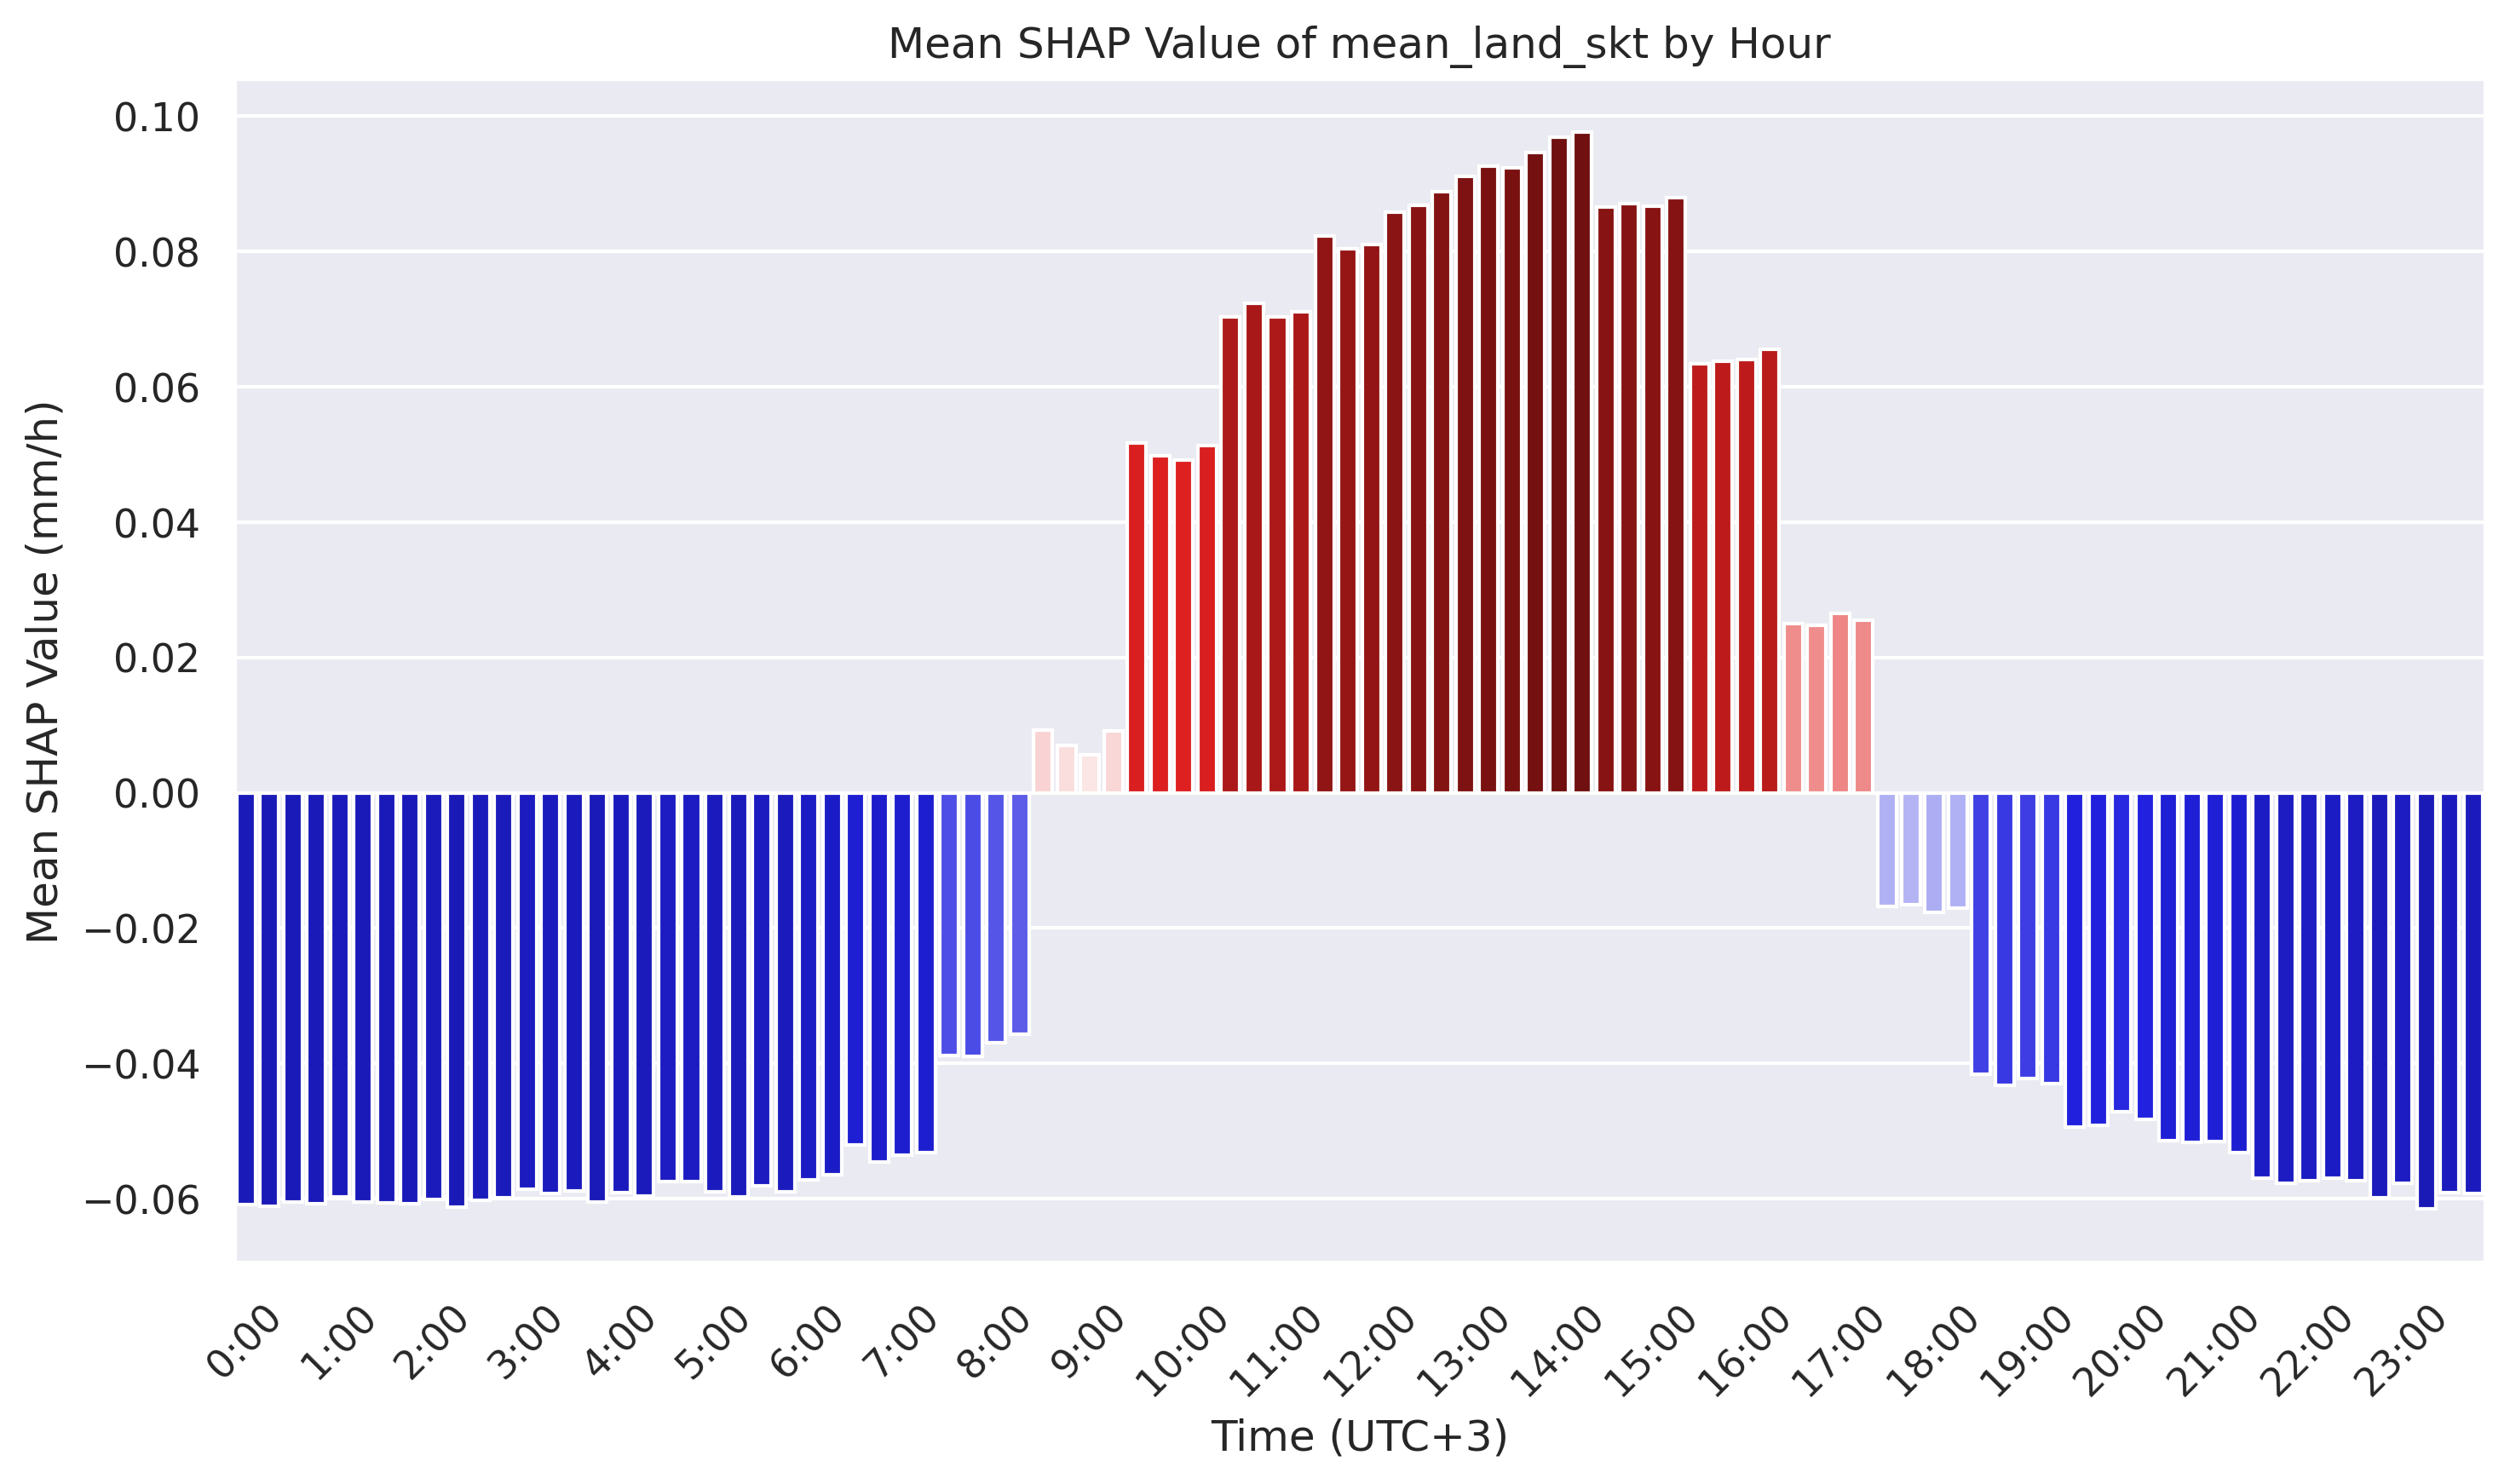
\includegraphics[width=\textwidth]{../figures/generated/experiments/obs_precipitation/temporal_corr/obs_precipitation_era5_shap_mean_land_skt_by_hour.png}
    \caption{Temporal variability of SHAP values for mean land skin temperature by hour for the \acrshort{era5} model predicting precipitation.}
    \label{fig:obs_precipitation_era5_shap_mean_land_skt_by_hour}
\end{figure}

Figure \ref{fig:obs_precipitation_era5_shap_domain_mean_cape_by_week_over_year} displays the change in contribution of domain mean \acrshort{cape} to precipitation by week over the year. The periods of high values in domain mean \acrshort{cape} correspond well with the two rainy seasons in the region. However, the contribution of domain mean \acrshort{cape} to precipitation is negative during these periods. As hinted at in Section \ref{sec:results-intensification}, this may suggest that when the overall atmospheric instability is high across the region, it may not be as conducive for individual storms to intensify or produce significant precipitation. Instead, more isolated pockets of high instability (i.e., high mean \acrshort{cape}) may be more favourable for fast intensification and/or heavy precipitation.

\begin{figure}[ht]
    \centering
    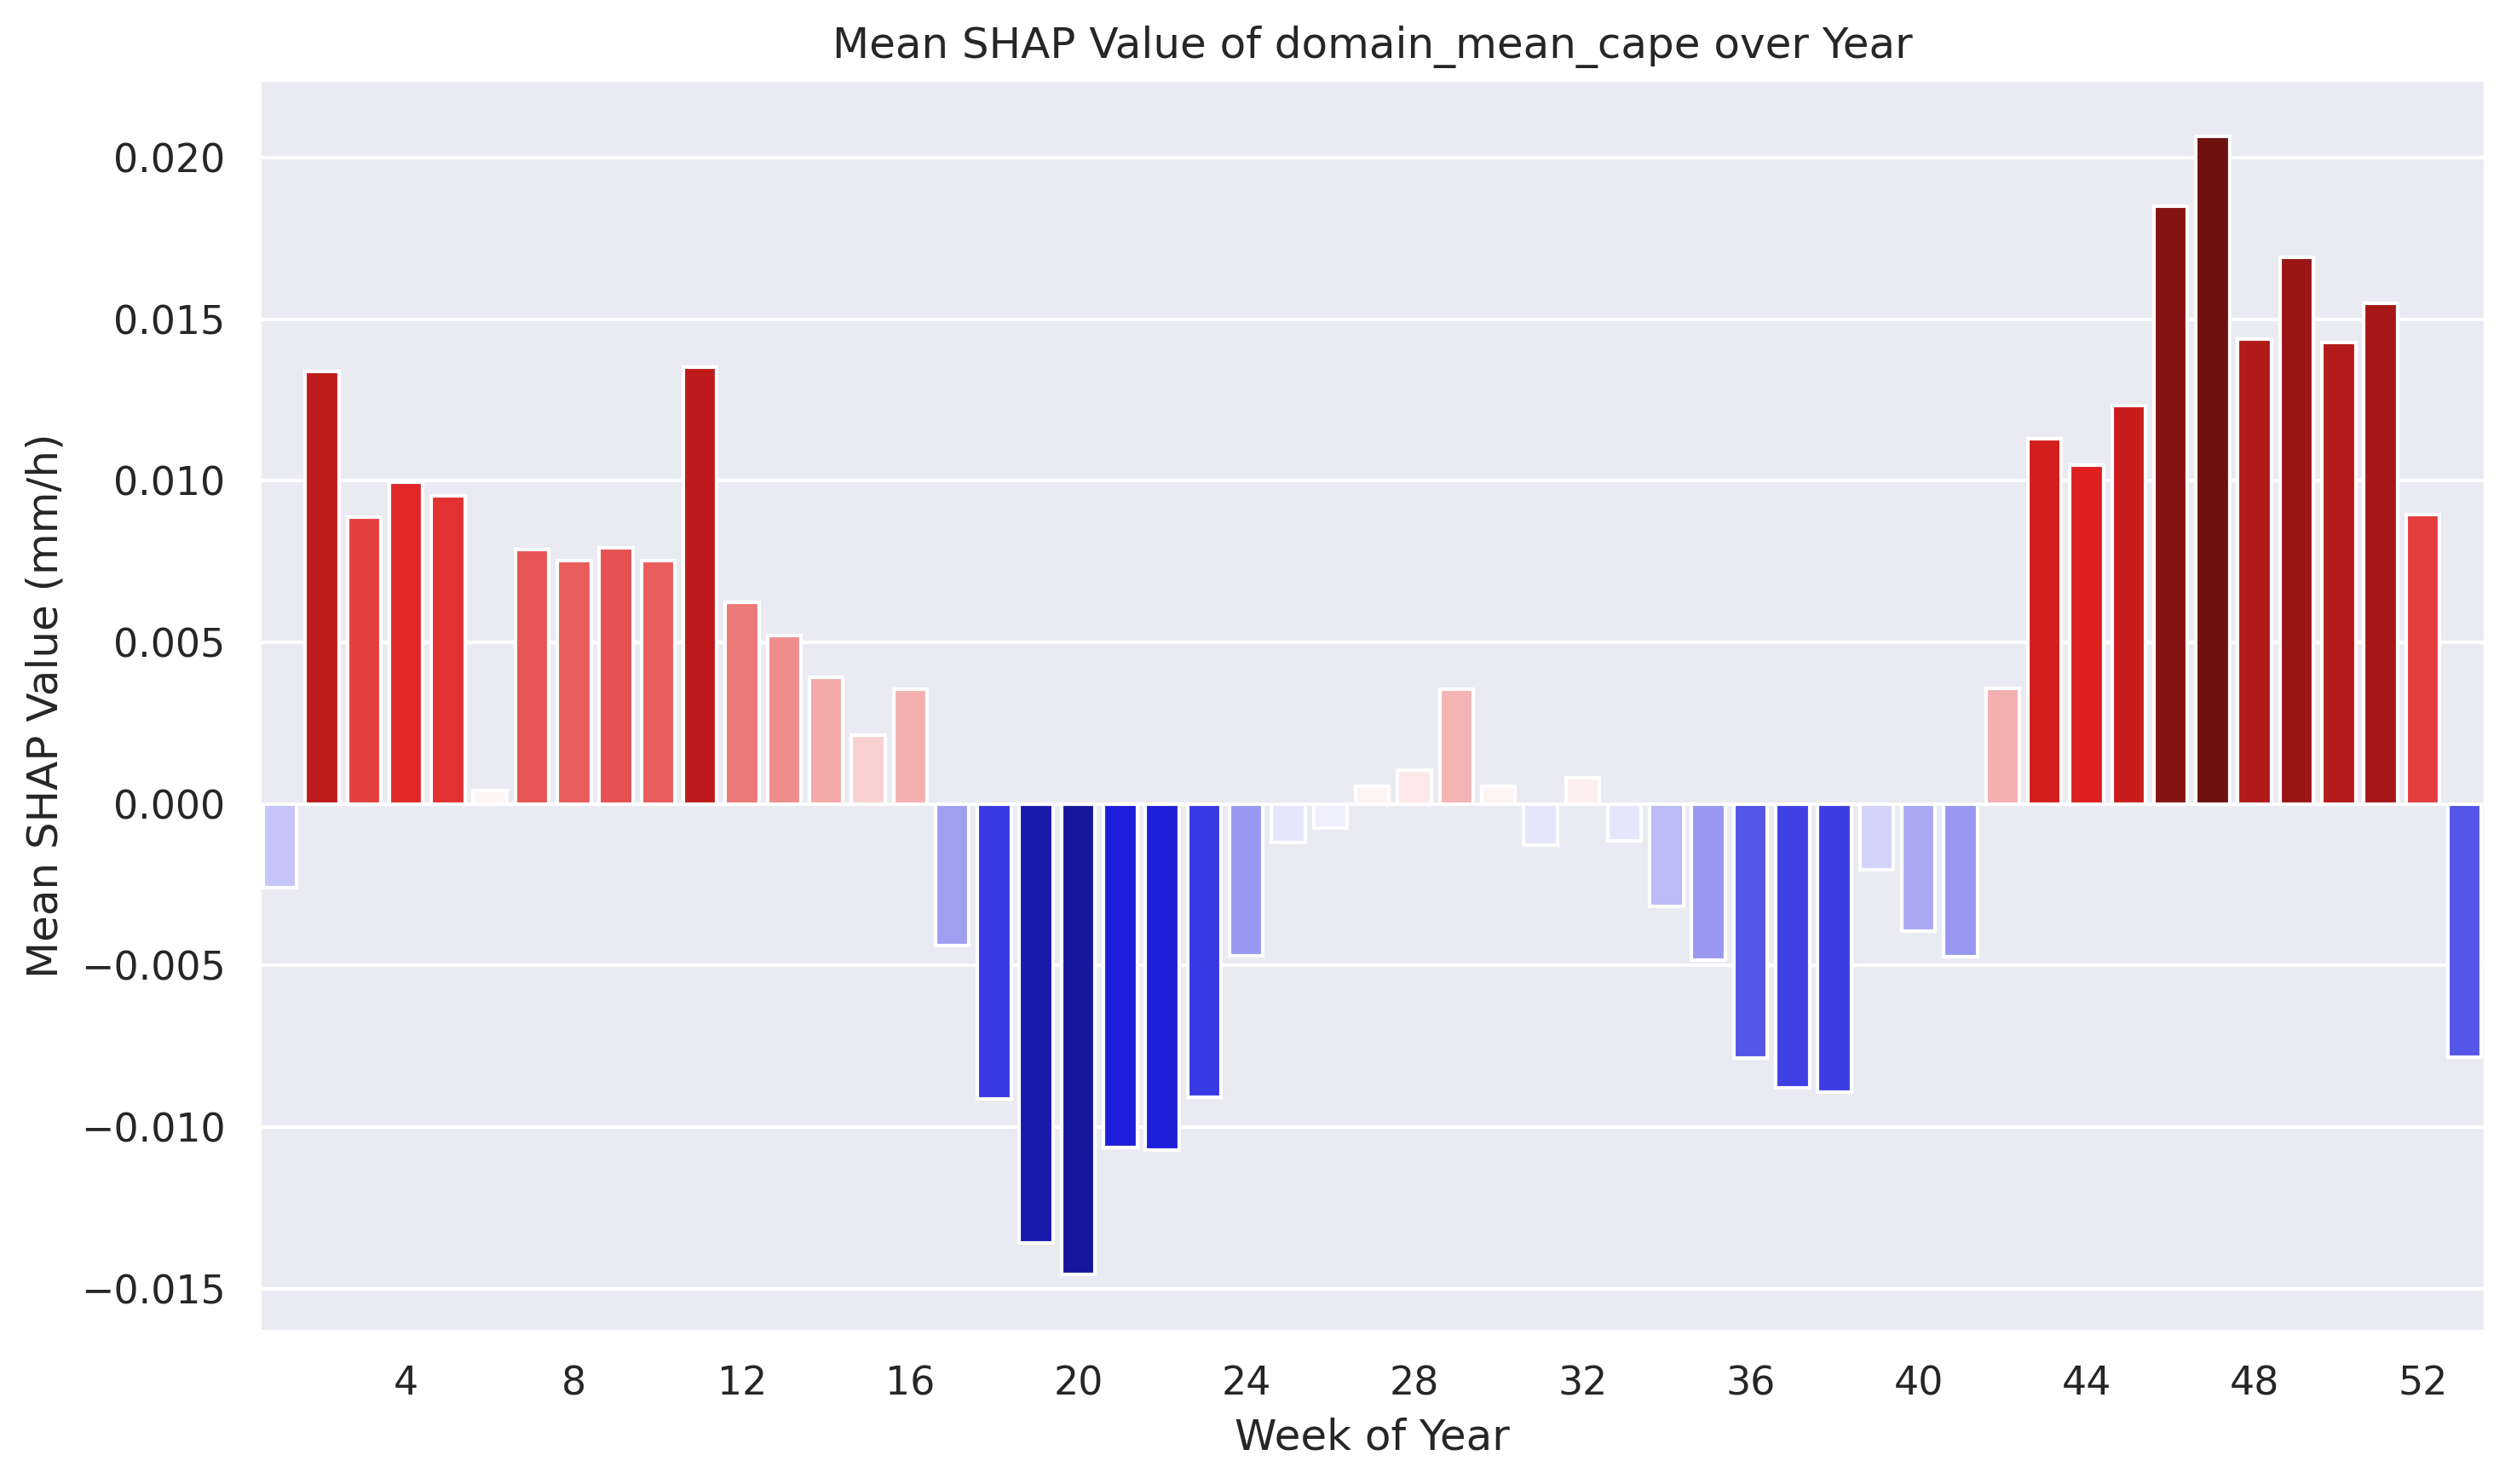
\includegraphics[width=\textwidth]{../figures/generated/experiments/obs_precipitation/temporal_corr/obs_precipitation_era5_shap_domain_mean_cape_by_week_over_year.png}
    \caption{Temporal variability of SHAP values for domain mean \acrshort{cape} by week over the year for the \acrshort{era5} model.}
    \label{fig:obs_precipitation_era5_shap_domain_mean_cape_by_week_over_year}
\end{figure}

It should be noted that the precipitation data has a direct relation with the predictands due to their common origin in the \acrshort{era5} data. This may lead to overfitting, as the models could learn to predict the precipitation values based on their inherent relationship with the storm characteristics rather than capturing the underlying physical processes. Indeed, we do observe that \acrshort{olr} has a high feature importance in the precipitation models, which is expected given its connection to the parametrisation schemes used for precipitation in \acrshort{era5} \citep{Hersbach2020}. This highlights the need for caution when interpreting the results and suggests that future work should consider incorporating independent precipitation datasets to validate the findings. For example, this thesis considered the inclusion of precipitation data from the Global Precipitation Measurement (GPM) mission, but ultimately did not include it due to over 70\% of storm observations lacking corresponding high-quality GPM data. A possible approach would be to recomputed the dataset using all available Integrated Multi-satellitE Retrievals for GPM (IMERG) data, regardless of quality, to increase coverage. While the availability of \acrshort{era5} data makes it a more practical choice for widespread application, the inclusion of other datasets would reduce interdependence between predictands and predictors, even if viable data coverage is reduced.